\documentclass[169, handout	]{THIbeamer} % for print add handout
\usepackage{biblatex}

\usepackage[utf8]{inputenc}
\usepackage[greek,ngerman]{babel}
\usepackage{hyperref}
\usepackage{multimedia}
\usepackage{csquotes}

% Table
\usepackage{hhline}
\usepackage{multirow}

% Figures
\usepackage{subcaption}
\captionsetup[subfigure]{justification=justified,singlelinecheck=false}
\graphicspath{{Images/}}

% Math
\usefonttheme[onlymath]{serif}
\usepackage{amsmath}
\usepackage{units}


% Tikz
\usepackage{tikz}
\usetikzlibrary{backgrounds,shadows,arrows}%external
\usepackage{pgfplots}
\usepackage{pgfgantt}
\usepackage{pdflscape}
\pgfplotsset{compat=newest}
%Only compile figures when something has changed
%\tikzexternalize[prefix=TikzPictures/]
\title{Ignaz Kögler Research Summer Camp}

\newcommand{\argmin}{\mathop{\mathrm{arg\,min}}}
\subtitle{KI \& Mobilität der Zukunft}

\date{01.03.2022}

%\author{Karthikeyan Chandra Sekaran}


\begin{document}
	\begin{frame}[plain]
		\maketitle
	\end{frame}
	\begin{frame}{Outline}
		\begin{minipage}{0.4\textwidth}
			\begin{enumerate}
				\item Einarbeitung in die Generierung von Echtdaten:
				\begin{enumerate}
					\item Grundlagen zur Aufzeichnung von Realdaten
					\item Robot Operating System (ROS)
				\end{enumerate}
				\item Datenvorverarbeitung:
				\begin{enumerate}
					\item Region of Interest
					\item Subtraktion der Bodenebene
					\item Clustering
					\item Objektliste
				\end{enumerate}
			\item[]
			\end{enumerate}
		\end{minipage}%
		\hfill
		\begin{minipage}{0.5\textwidth}
		\begin{tabular}{p{\textwidth}}
			\begin{enumerate}
				\setcounter{enumi}{2}	
				\item KI-Methoden: 				
				\begin{enumerate}
					\item Grundlagen der künstlichen Intelligenz					
					\item Ermittlung der Kritikalität	
				\end{enumerate}	
				\item Online-Verwendung der KI-Methoden
			\end{enumerate}
		\end{tabular}
		\end{minipage}%
	\end{frame}
\begin{frame}{Einarbeitung in die Generierung von Echtdaten}{Grundlagen zur Aufzeichnung von Realdaten}
	\textbf{Szenariobeschreibung:}\\
	Zwei Fahrzeuge fahren auf der gleichen Spur, in der gleichen Richtung und mit einer ähnlichen konstanten Geschwindigkeit. Das vorausfahrende Fahrzeug führt eine Vollbremsung durch.\\
	\textbf{Forschungsfrage:} \\
	Wie könnte man einen Unfall verhindern?.\\
Welche Informationen werden benötigt, um eine Entscheidung zu treffen?.
\end{frame}
	\begin{frame}{Einarbeitung in die Generierung von Echtdaten}{Grundlagen zur Aufzeichnung von Realdaten}
Viele Fahrzeuge sind mit externen Sensoren, wie Radar und Kameras, ausgestattet. Und viele Unternehmen (wie z. B. Velodyne oder Valeo) entwickeln LiDAR-Sensoren für die Automobilbranche.\\
Unter der Annahme, dass einige Zustandsgrößen des Fahrzeugs bekannt sind, z. B. seine Geschwindigkeit über Grund und seine Längsbeschleunigung, ist es möglich, die Zeit bis zur Kollision (engl. Time To Collision - TTC) $t_{\text{ttc}}$ zu schätzen.\\
		\textbf{Ziele:} \\
Eine KI-Methode zu programmieren, die es erlaubt, die TTC eines Fahrzeugs zu schätzen. 
	\end{frame}
\begin{frame}{Einarbeitung in die Generierung von Echtdaten}{Grundlagen zur Aufzeichnung von Realdaten}
	\textbf{Vorgeschlagenes Verfahren:} \\
	Ein Testfahrzeug mit hochmodernen Sensoren auszustatten: einen Automotive Dynamic Motion Analyzer (ADMA), a Correvit S-Motion and a LiDAR.
	\textbf{Vorteile:} \\
	\begin{enumerate}
		\item Hochpräziser Fahrzeugzustand (Position, Geschwindigkeit, Orientierung, Beschleunigungen usw.).
		\item Hochpräzise Informationen über die Umgebung, inkl. andere Fahrzeuge.
		\item Zusätzlich können die Fahrzeuginformationen von den bordeigenen Sensoren abgerufen werden.
	\end{enumerate}
\end{frame}
		\begin{frame}{Einarbeitung in die Generierung von Echtdaten}{Grundlagen zur Aufzeichnung von Realdaten}
		\begin{figure}
			\centering
			\begin{subfigure}[b]{0.4\textwidth}
				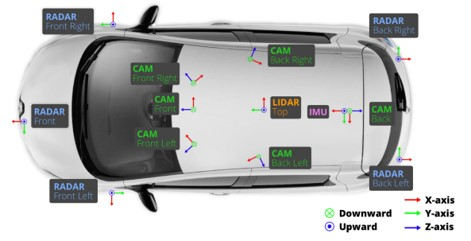
\includegraphics[scale=0.4]{required/Sensorkoordinatensysteme.jpg}
				\caption{Sensorkoordinatensysteme in nuScenes [Caesar.2020]}
				\label{ROS}
			\end{subfigure}
			\vfill
			\begin{subfigure}[b]{0.4\textwidth}
				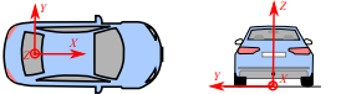
\includegraphics[scale=0.5]{required/Fahrzeugkoordinatensystem exterozeptiver Sensoren.jpg}
				\caption{Fahrzeugkoordinatensystem exterozeptiver Sensoren}
				\label{ROS}
			\end{subfigure}
			\hspace{1.5 cm}
			\begin{subfigure}[b]{0.4\textwidth}
				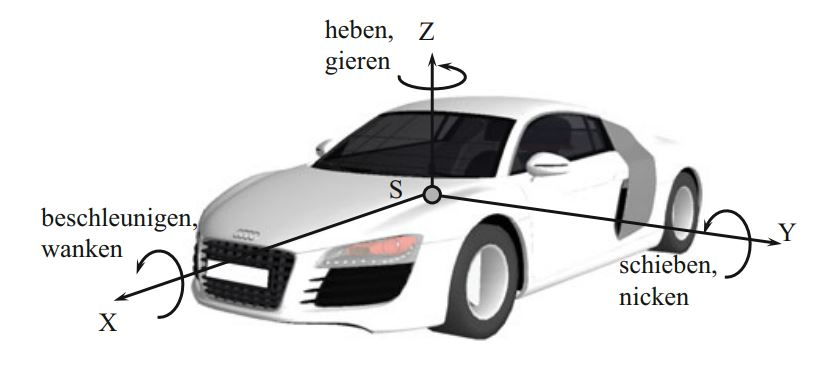
\includegraphics[scale=0.2]{required/Fahrzeugkoordinatensystem CoG.jpg}
				\caption{Fahrzeugkoordinatensystem der Fahrdynamikgleichungen [Breuer.2015]}
				\label{ROS}
			\end{subfigure}
		\end{figure}
		
	\end{frame}
	\begin{frame}{Einarbeitung in die Generierung von Echtdaten}{Grundlagen zur Aufzeichnung von Realdaten}
		\begin{itemize}
			\item \textbf{LiDAR} steht als Akronym für \enquote{Light Detection And Ranging}.
			\item Es ist ein optisches Verfahren zur Messung von Distanzen.
			\item Es sendet Laserlicht in Pulsen aus und misst die Flugzeit des Pulses.
			\item Es arbeitet mit Wellenlängen nahe des sichtbaren Bereichs ($\mu m$-Wellen).
		\end{itemize}
		Gezeigt ist eine visualisierung des Lidar-Prinzips[Wik.2022]:
		\begin{figure}[htbp]
    		\centering
    		\begin{subfigure}[b]{0.15\textwidth}
        		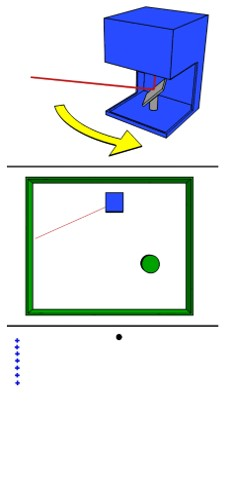
\includegraphics[scale=0.21]{required/LiDAR-Sensor1.jpg}
        		\label{Lidar-t1}
   		 	\end{subfigure}
    		\begin{subfigure}[b]{0.15\textwidth}
       		 	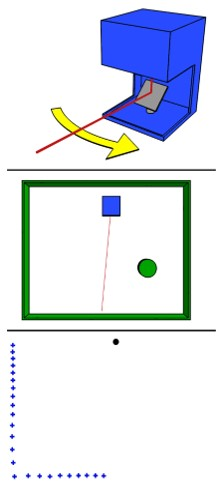
\includegraphics[scale=0.21]{required/LiDAR-Sensor2.jpg}
        		\label{Lidar-t2}
    		\end{subfigure}
   	 		\begin{subfigure}[b]{0.15\textwidth}
        		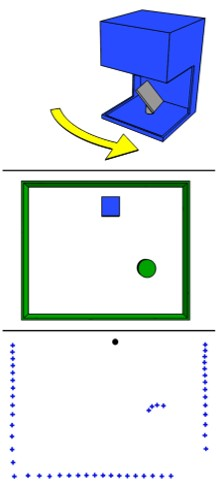
\includegraphics[scale=0.21]{required/LiDAR-Sensor3.jpg}
        		\label{Lidar-t3}
    		\end{subfigure}
    		\label{Lidar in Raum}
		\end{figure}
	\end{frame}
	
	\begin{frame}{Einarbeitung in die Generierung von Echtdaten}{Grundlagen zur Aufzeichnung von Realdaten}
		\begin{itemize}
			\item \textbf{Distanzmessung} per \enquote{time-of-flight}-Prinzip:
			\begin{itemize}
				\item Sende- $t_\text{send}$ und Empfangszeit $t_\text{back}$ des Pulses wird gemessen, d.h., die Zeit, die der Puls braucht, um ein Objekt zu erreichen und zum LiDAR zurückgeworfen zu werden.
				\item Aus der Zeitdifferenz $\Delta t_\text{L}=t_\text{back}-t_\text{send}$ und der Geschwindigkeit des Lichts $ c = 3 \cdot 10^{8} \frac{m}{s} $.
				\begin{equation}
					r = \frac{c}{2} \cdot \delta t
				\end{equation}
			\end{itemize}
			\item \textbf{Geschwindigkeitsbestimmung:} Auf Basis von Signalverarbeitungstechniken aus der Distanzmessung ableitbar.
			\item \textbf{Vorteile}: Großer Öffnungswinkel, Detektion aller möglichen Objekte (ohne Training, da aktiver Sensor), Klassifizierung von Objekten möglich, etc.
			\item \textbf{Nachteile:} Wetteranfälligkeit, keine direkte Geschwindigkeitsmessung.
		\end{itemize}
	\end{frame}
	\begin{frame}{Einarbeitung in die Generierung von Echtdaten}{Grundlagen zur Aufzeichnung von Realdaten}
		\begin{itemize}
			\item \textbf{Ausgabeformat:} [$x, y, z, int, t$] $\rightarrow$ $N \times 5$ Matrix für eine Punktwolke mit $N$ Punkten
			\item \textbf{Speicheranforderungen:} Als Beispiel, der Velodyne HDL-64E (rotierender 3D Laserscanner, der z.B. im  Open-Source Kitti-Datensatz verwendet wird):
			\begin{itemize}
				\item Sichtfeld: 360° horizontal, 36.8° vertikal | Reichweite: 120 m | Frequenz: 10 Hz
				\item Ausgegebene Punkte: $~ 1.3 \cdot 10^{6}$ $\frac{\text{pts}}{\text{s}}$ 
				\item Benötigter Speicher: $~1.8$ $\frac{\text{MB}}{\text{Frame}} \cdot 10$ $\frac{\text{Frames}}{\text{s}} = 18$  $\frac{\text{MB}}{\text{s}}$
			\end{itemize}			 
			\item \textbf{Beispiel:}
		\end{itemize}					
		\begin{figure}
			\includegraphics[scale=0.3]{required/LiDAR auf Parkplatz.jpg}
			\caption{LiDAR-Aufnahme auf einem Parkplatz [Rummelhard.2017]}
		\end{figure}
	\end{frame}
	\begin{frame}{Einarbeitung in die Generierung von Echtdaten}{Grundlagen zur Aufzeichnung von Realdaten}	
		\begin{itemize}
			\item \textbf{ADMA} steht als Akronym für \enquote{Automotive Dynamic Motion Analyzer}
			\item Er setzt sich aus Inertialmesssystem (engl. Inertial Measurement Unit - IMU), Satellitennavigation (engl. Global Navigation Satellite System - GNSS) und einem Prozessor zusammen, und kann somit Geschwindigkeit, räumliche Lage des Fahrzeugs und Standort in Echtzeit ausgeben.
		\end{itemize}
		\begin{figure}
			\centering
    		\begin{subfigure}[b]{0.3\textwidth}
				\includegraphics[scale=0.3]{required/ADMA-Erklärung.jpg}
				\caption{ADMA als \enquote{Sinnesorgan} des Fahrzeugs [AD14]}
        		\label{ADMA Erklärung}
   		 	\end{subfigure}
   		 	\hspace{3cm}
    		\begin{subfigure}[b]{0.3\textwidth}
				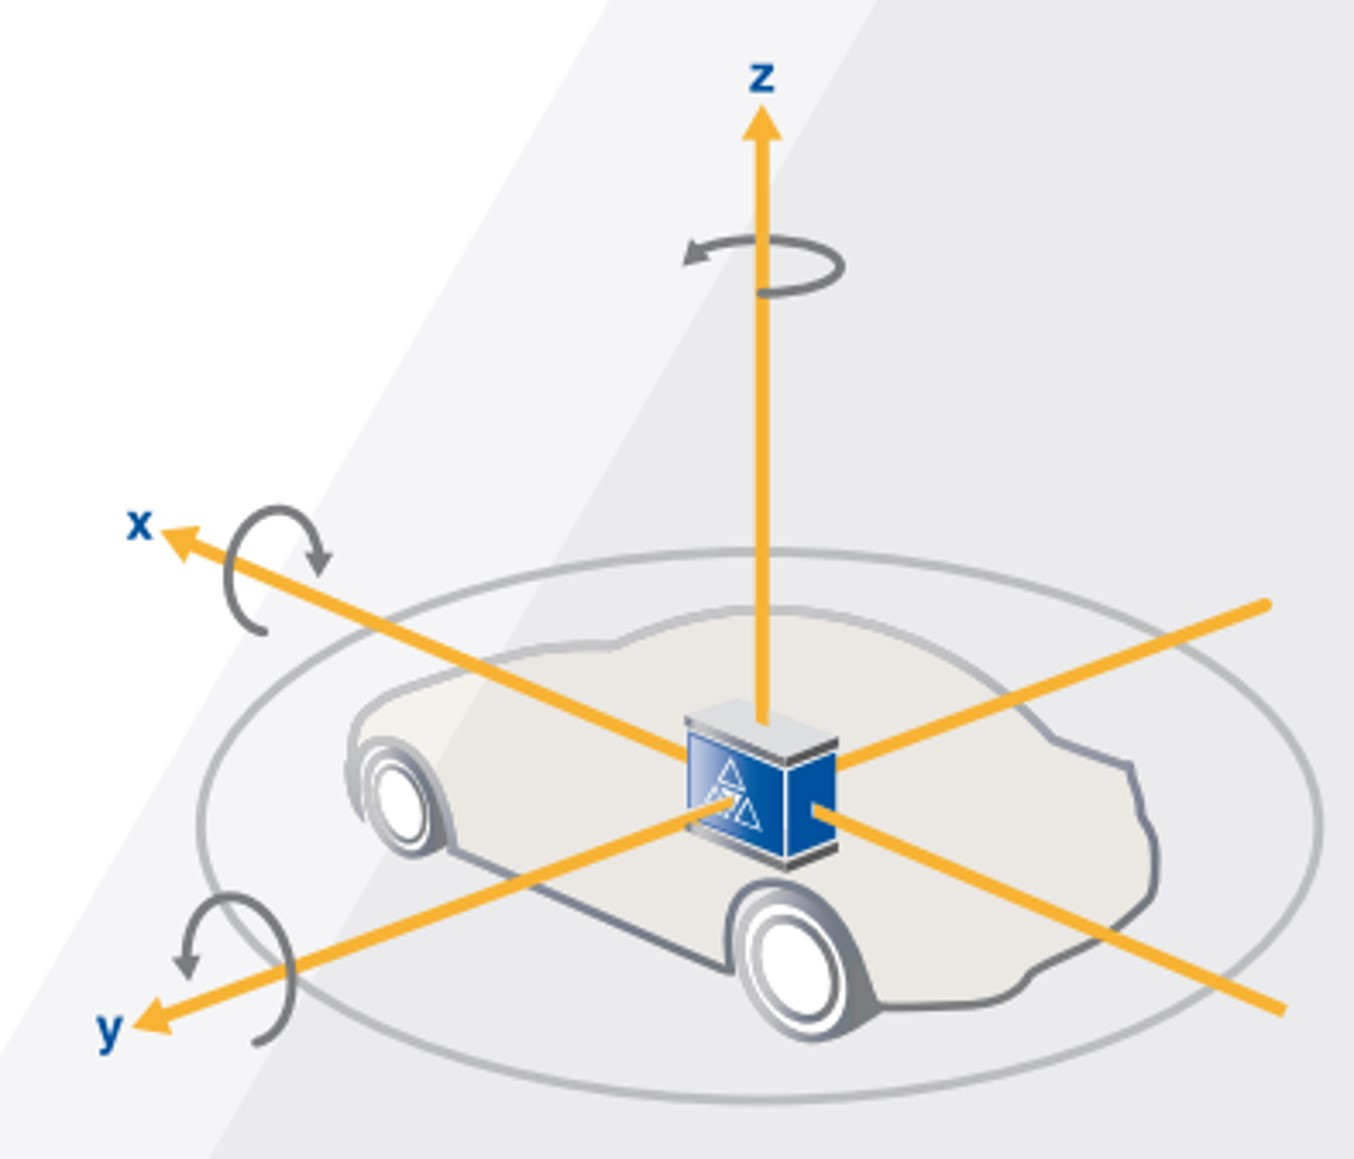
\includegraphics[scale=0.3]{required/ADMA.jpg}
				\caption{ADMA im Fahrzeug [GeneSys.2022]}
        		\label{ADMA in Fahrzeug}
    		\end{subfigure}
    		\label{ADMA figures} 
		\end{figure}
	\end{frame}

	\begin{frame}{Einarbeitung in die Generierung von Echtdaten}{ROS}
		Die Arbeit mit realen Daten hat jedoch ihre Herausforderungen:
		\begin{itemize}
			\item Die Menge des benötigten Speicherplatzes kann schnell wachsen, besonders bei Verwendung mehrerer Sensoren.
			\item Selbst High-End-Sensoren führen keine fehlerfreien Messungen durch: Ein Sensorrauschen ist immer vorhanden.
			\item Eine Koordinatentransformation kann erforderlich sein, wenn mehrere Sensoren verwendet werden.
			\item Abhängig davon, u.a. ob die Zustandsvariablen getrackt werden, kann eine Sensorfusion erforderlich sein.
		\end{itemize}
	\end{frame}
%\begin{frame}{Einarbeitung in die Generierung von Echtdaten}{ROS}
%	\textbf{Solutions:} 
%	\begin{itemize}
%		\item \textcolor{purple}{remove floor}
%		\item \textcolor{purple}{cluster}
%		\item \textcolor{purple}{track? }
%		\item Filtern von störenden oder für den Verwendungszweck nicht relevanten Anteile.
%		\item Algorithmus-Optimierung für die Reduzierung des Speicher- und Rechenbedarfs.
%		\item Nutzen von A-Priori Wissen zur Verkleinerung des ausgewerteten Lösungsraums.
%		\item Erfüllung der Echzeitanforderungen
%	\end{itemize}
%	\textbf{Aufgabenstellung:} Ausgabe der Punktewolke für die wichtigen Objekte der Aufnahme
%\end{frame}
%	\begin{frame}{Datenvorverarbeitung}{Erläuterung}
%		\textbf{Vorgehensweise:} 
%		\begin{enumerate}
%			\item \enquote{Region of Interest}-Filterung: Filterung der für den Verwendungszweck unrelvanten Daten
%			\item \enquote{Ground Subtraction}: Filterung der Lidarpunkte der Fahrbahnfläche
%			\item \enquote{Clustering}: Segmentierung zusammenhängender Punkte 
%			\item \enquote{Objekterkennung}: Ausgabe von Objekten auf Basis der Clustergrenzen
%		\end{enumerate}
%		\vspace{0.5cm}
%		Eine genauere Erläuterung zu den einzelnen Schritten wird in den folgenden Kapiteln gegeben.
%	\end{frame}	
\begin{frame}{Einarbeitung in die Generierung von Echtdaten}{ROS}
	\textbf{Vorgehensweise:} 
	\begin{enumerate}
		\item \enquote{Region of Interest}-Filterung: Reduzierung der benötigten Speicher- und Rechenleistung durch Begrenzung der zu messenden Fläche.
		\item \enquote{Subtraktion der Bodenebene}: Reduzierung der benötigten Speicher- und Rechenleistung durch Ausblenden irrelevanter Daten (Fahrbahnfläche).
		\item \enquote{Clustering}: Bestimmte Messungen gruppieren, um sie als ein einziges Objekt und nicht als mehrere Punkte zu betrachten.
		\item \enquote{Objektverfolgung}: Mobile Objekte in der Umgebung des Fahrzeugs zu verfolgen. 
	\end{enumerate}
\end{frame}
	\begin{frame}{Einarbeitung in die Generierung von Echtdaten}{ROS}			
		Der Algorithmus wird in Robot Operating System (ROS) implementiert:
		\begin{itemize}
			\item bietet Struktur, Tools und Algorithmen für die Implementierung eigener Applikationen.
			\item die Sensorausgabe kann in dieses System eingebunden und somit verarbeitet werden.
			\item Open-Source Framework.
		\end{itemize}		
		\begin{figure}
			\centering
    		\begin{subfigure}[b]{0.4\textwidth}
				
\includegraphics[scale=0.3]{required/ROS.jpg}
				\caption{ROS: Noetic Ninjemys [ROS.2022]}
        		\label{ROS}
   		 	\end{subfigure}
    		\begin{subfigure}[b]{0.4\textwidth}
				
\includegraphics[scale=0.3]{required/ROS2.jpg}
				\caption{ROS 2: Humble Hawksbill [ROS.2022]}
        		\label{ROS}
    		\end{subfigure}
		\end{figure}			
	\end{frame}
\begin{frame}{Einarbeitung in die Generierung von Echtdaten}
	\begin{figure}
		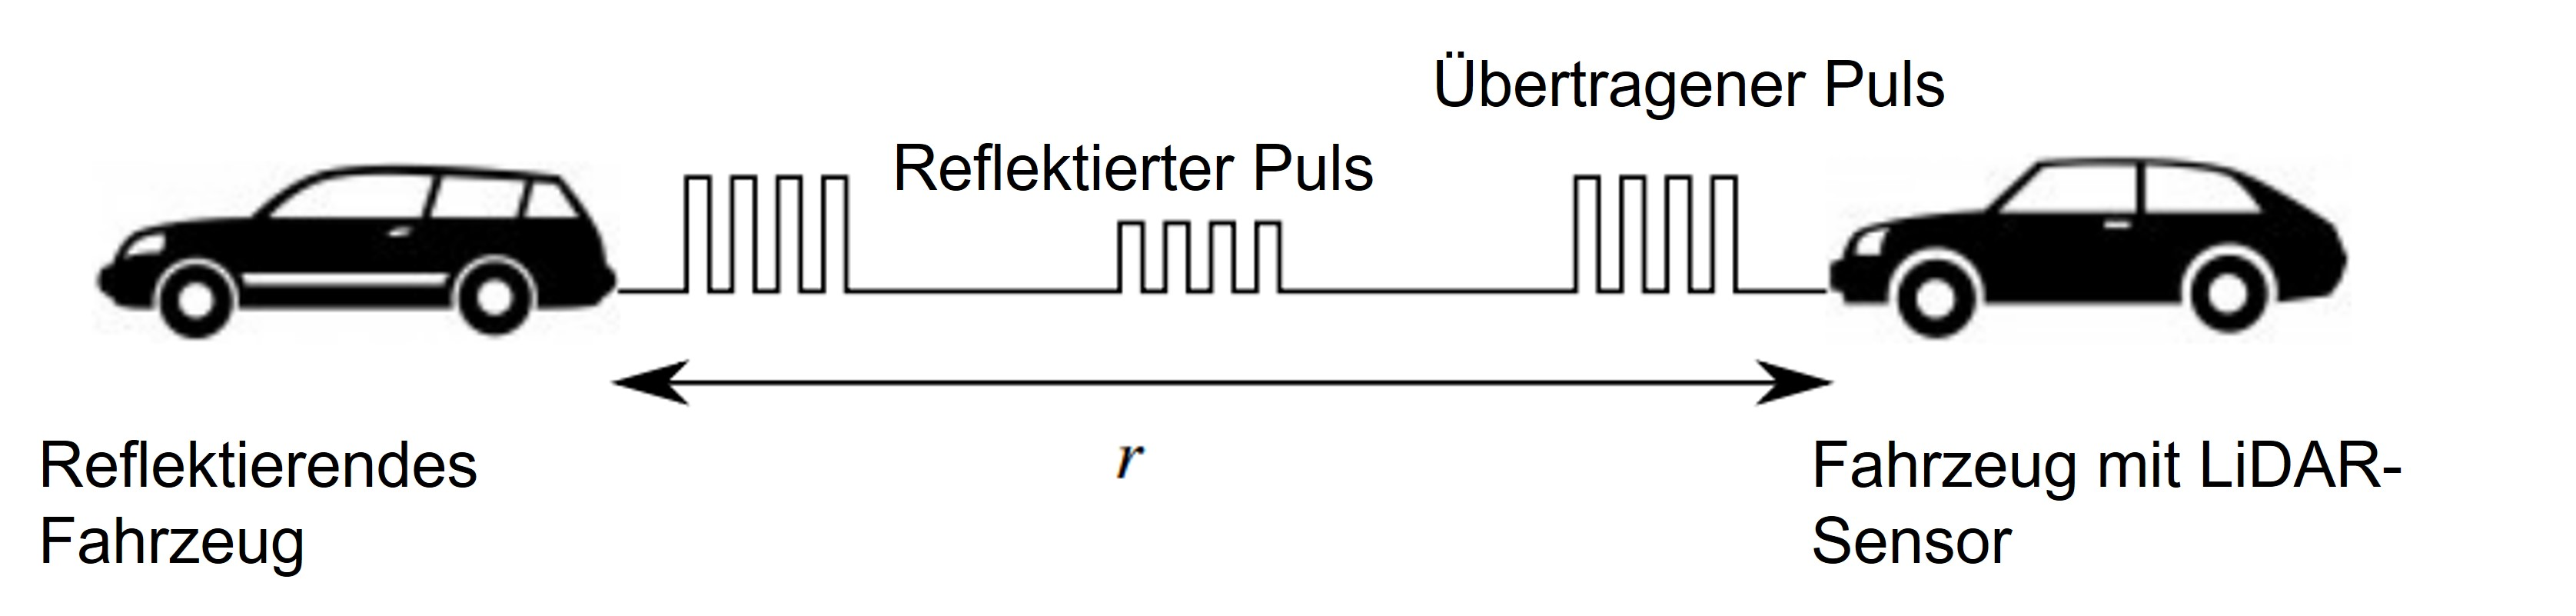
\includegraphics[scale=0.4]{"required/Szenariobeschreibung_auto.jpg"}
	\end{figure}	
	\textbf{Gedankenexperiment:}\\
	\begin{enumerate}
		\item Welche weiteren Fahrerassistenzsysteme sind bei einem Fahrzeug mit dieser Ausstattung denkbar? 
	\end{enumerate}
\end{frame}
	\begin{frame}{Einarbeitung in die Generierung von Echtdaten}{ROS}			
		\footnotesize
		ROS als Betriebssystem hat verschiedene Komponenten:
		\begin{itemize}
			\item \textbf{Nodes}: Prozesse, die eine bestimmte Aufgabe erfüllen.
			\item \textbf{Topics}: eigener \enquote{Kommunikationskanal}. Wird für den Informationsaustausch verwendet
			\item \textbf{Messages}: Enthalten die Informationen, die von den Knoten generiert und/oder konsumiert werden und die über die Topics ausgetauscht werden.
			\item \textbf{Master}: Zentraler Knotenpunkt des Systems. Kennt alle Knoten, Topics und Messages. Koordiniert den Informationsaustausch und die Ausführung der Knoten.
			\item Programmiersprachen: C++, Python 
		\end{itemize}				
		\begin{figure}
			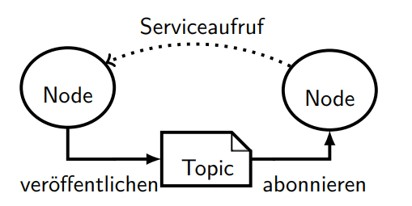
\includegraphics[scale=0.35]{required/ROS-Aufbau.jpg}
			\caption{Darstellung der Kommuikation zwischen Nodes in ROS}
		\end{figure}
	\end{frame}
\begin{frame}{Datenvorverarbeitung}{Region of Interest}
	\begin{itemize}
		\item Zahlreiche Koordinatensysteme im Fahrzeug, die eine Betrachtung der Information aus verschiedenen Perspektive ermöglichen.
		\item Zwischen den lokalen Koordinatensystemen des Fahrzeugs kann ein statischer Zusammenhang, analog einer Starrkörperbewegung, angenommen werden $\rightarrow$ Transformationsmatrizen sind zeitunabhängig.
		\item Fahrzeugkoordinatensysteme sind bei der Berechnung zwingend zu beachten, da Sie den Variablen Bedeutung verleihen.
		%			\item Beispiel einer Fahrdynamikgleichung:
		%			\begin{equation}
			%				\hspace*{0.2em}^V\vspace*{-0.2em}v_{x} = \frac{\delta}{\delta t}x \text{ gilt für } x =\hspace*{0.2em}^V\vspace*{-0.2em}x
			%			\end{equation}
		%					
	\end{itemize}
\end{frame}
\begin{frame}{Datenvorverarbeitung}{Region of Interest}
	\begin{figure}
		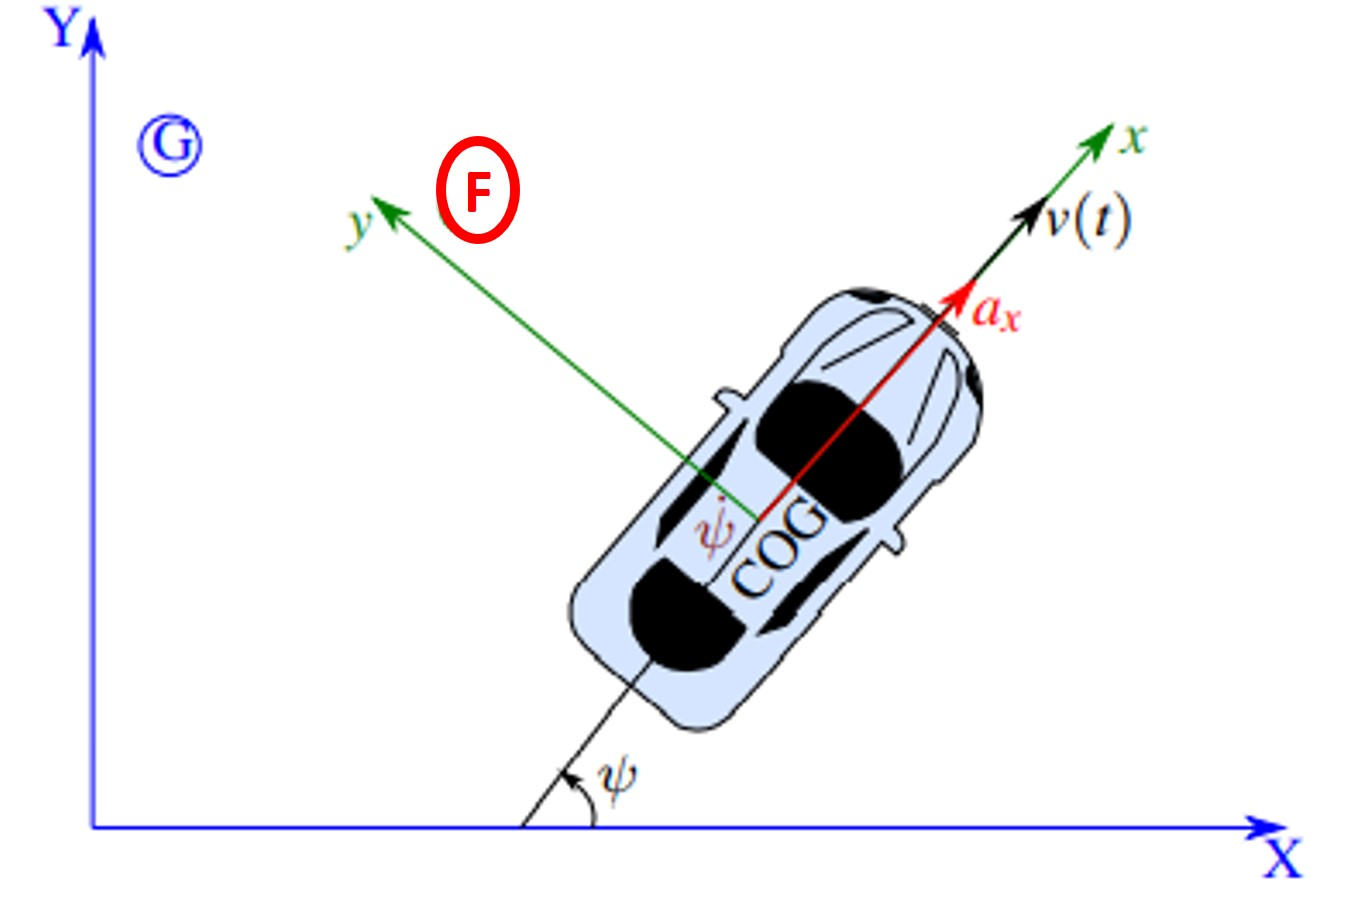
\includegraphics[scale=0.3]{required/Globales Koordinatensystem.jpg}
		\caption{Dargestellt ist ein Fahrzeug in einem globalen Koordinatensystem.}
		\label{Globales Koordinatensystem}
	\end{figure}
	\begin{itemize}
		\item Die Daten aller Sensoren werden in ein Stationäres Referenzkoordinatensystem umgewandelt.
		\item Ermöglicht die Beschreibung von Objekten relativ zu einem konstanten Koordinatensystem.
		\item Transformationsmatrix von lokalem Fahrzeugkoordinatensystem zu globalem Koordinatensystem ist für instationäre Objekte zeitabhängig.
	\end{itemize}					
\end{frame}
\begin{frame}{Datenvorverarbeitung}{Region of Interest}
	\textbf{Nomenklatur:} 
	\begin{itemize}
		\item $\hspace*{0.2em}^E\vspace*{-0.2em}P$ : Punkt im globalen Koordinatensystem
		\item $\hspace*{0.2em}^L\vspace*{-0.2em}P$ : Punkt im LiDAR Koordinatensystem
		\item $\hspace*{0.2em}^V\vspace*{-0.2em}P$ : Punkt im Fahrzeugkoordinatensystem (CoG)
		\item $\hspace*{0.2em}^{S}\vspace*{-0.2em}P$ : Punkt im Fahrzeugkoordinatensystems der exterozeptiven Sensoren
	\end{itemize}
\end{frame}
\begin{frame}{Datenvorverarbeitung}{Region of Interest}
	\begin{figure}
		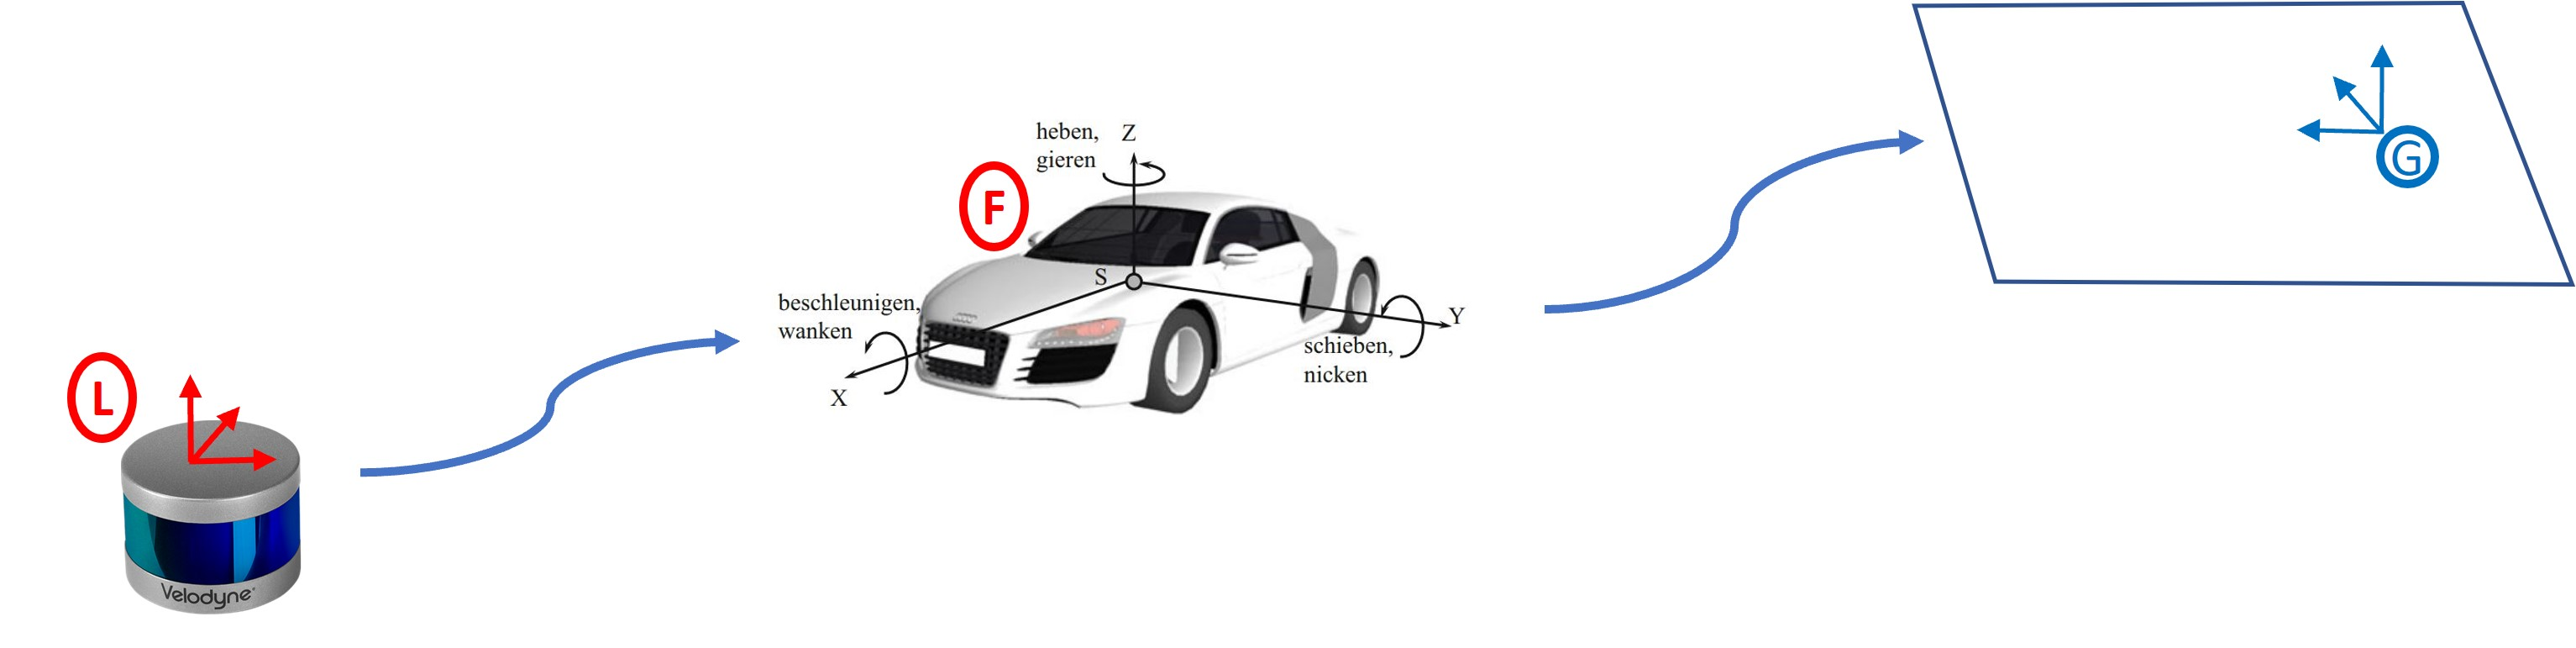
\includegraphics[scale=0.5]{required/Szenarioanwendung Koordinatentransformation.jpg}
		\caption{Die Abbildung zeigt eine grafische Darstellung der Koordinatentransformation vom LiDAR-Koordinatensystem in das Fahrzeugkoordinatensystem und vom Fahrzeugkoordinatensystem in das globale Koordinatensystem. Zusammengesetzt aus Abbildungen in [Breuer.2015] und [Velodyne.2020]}
		\label{Globales Koordinatensystem}
	\end{figure}
	\footnotesize
	%       	\begin{itemize}
		%       		\item Innerhalb des Fahrzeug: statische Koordinatentransformation 
		%       		\item Zwischen Fahrzeug- und Erdkoordinatensystem: zeitabhängige Koordinatentransformation (Position des Fahrzeugs im globalen Koordinatensystem durch den ADMA-Sensor gegeben)
		%			\item Umsetzung mit tf-Modul aus ROS
		%       	\end{itemize}
	
	
\end{frame}
\begin{frame}{Datenvorverarbeitung}{Region of Interest}
	\footnotesize
	\begin{itemize}
		\item Das ROS-Pachage \enquote{tf} liefert als Output die Transformationsmatrix zwischen Referenzsystemen.
		\item Das RVIZ ROS-Package wird zur Visualisierung der transformierten Messungen verwendet.
		\item RVIZ zeigt die transformierten Messungen an, wie sie vom tf-Package erzeugt wurden (see tutorial 2).
		%			\item Unterteilung in statische und dynamische (zeitabhängige) Transformatoren wird mit den jeweiligen Transformatoren umgesetzt
	\end{itemize}
	\textbf{Tutorial Links}
	\begin{enumerate}
		\item http://wiki.ros.org/tf/Tutorials
		\item http://wiki.ros.org/tf/Tutorials/Introduction\%20to\%20tf
		\item http://wiki.ros.org/tf2
		\item Youtube-Tutorial: https://www.youtube.com/watch?v=QyvHhY4Y\_Y8
	\end{enumerate}

\textcolor{blue}{**s. coordinate transformation code**}

\end{frame}
%	\begin{frame}{ROS}{Ordnerstruktur}
%		\begin{figure}
%			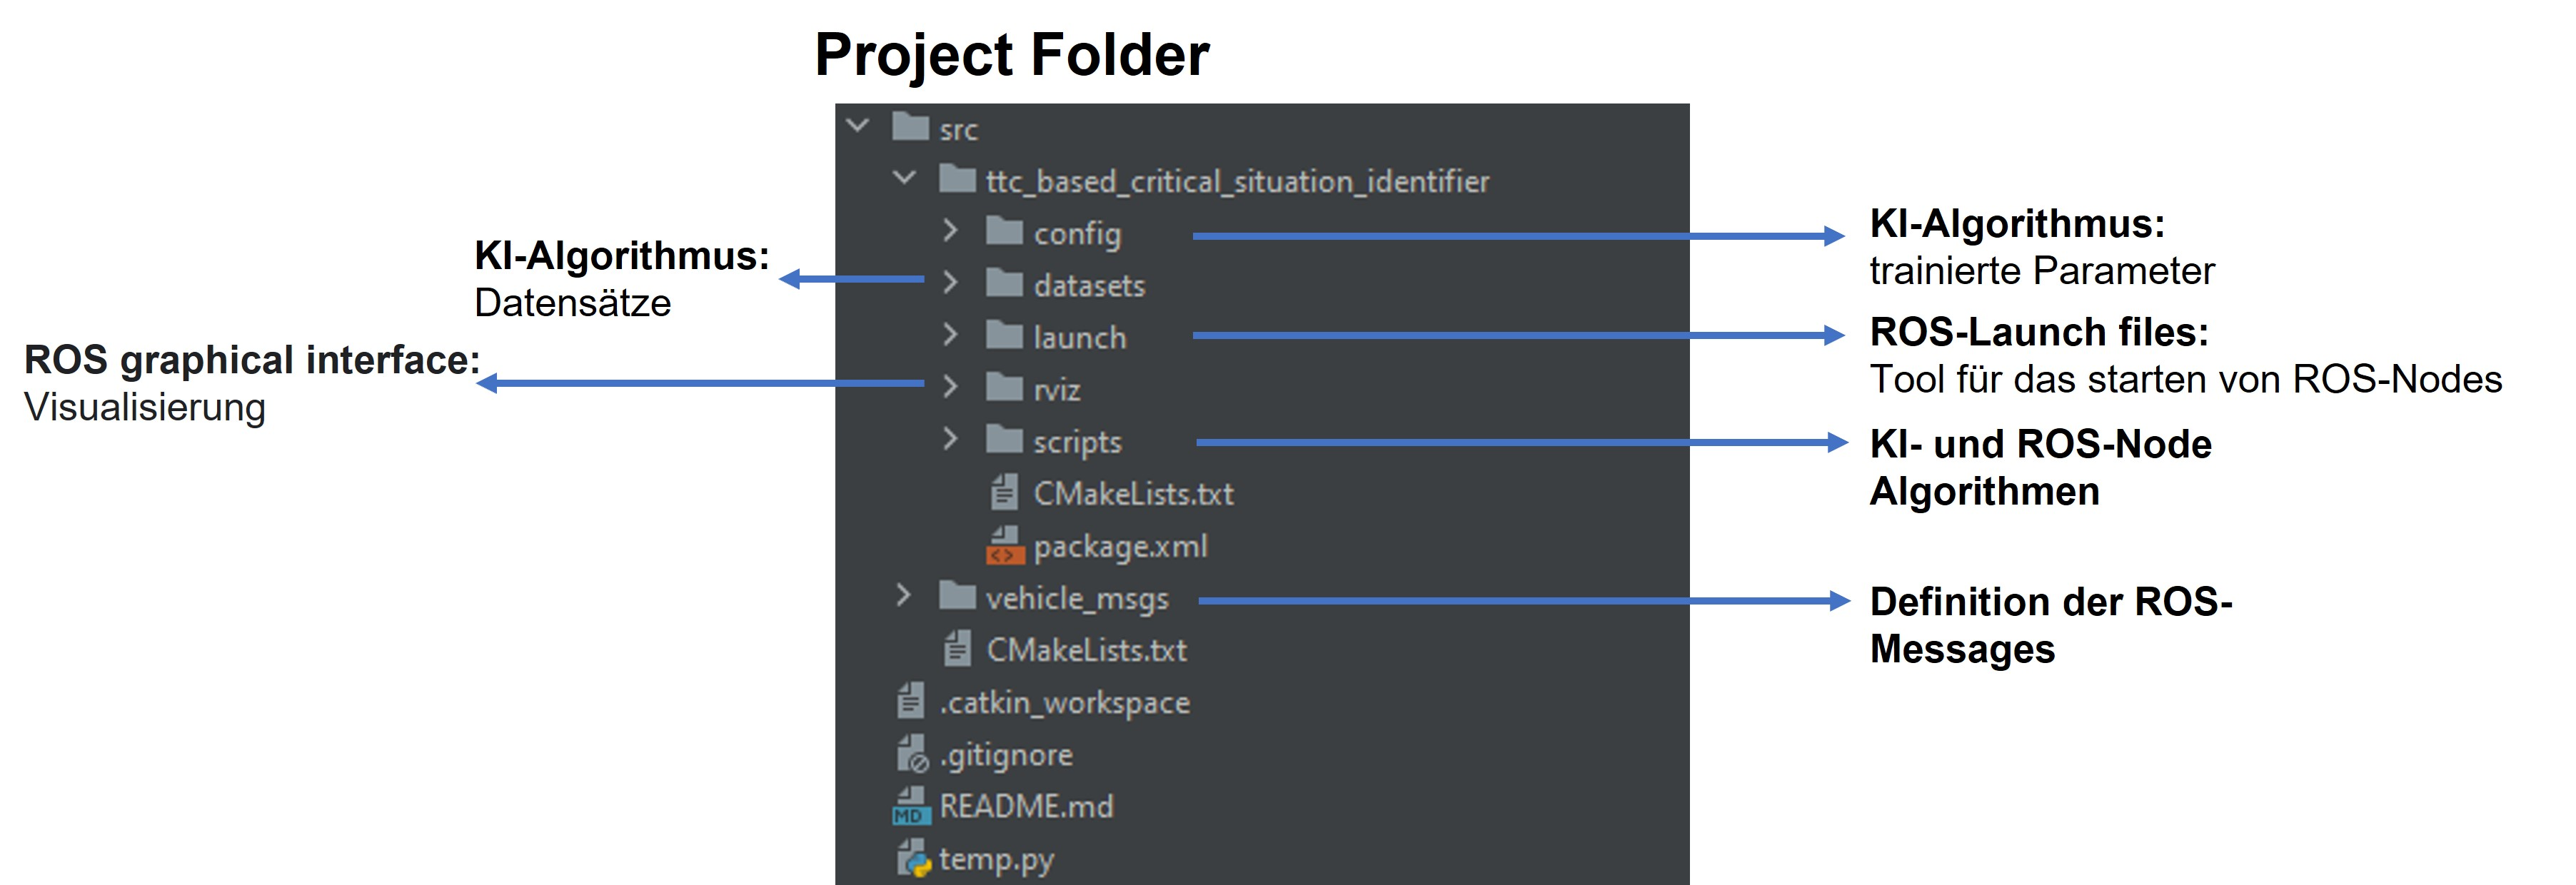
\includegraphics[scale=0.5]{required/ROS_Folder_Structure.jpg}
%			\caption{Darstellung der Ordnerstruktur}
%		\end{figure}
%	\end{frame}
%	\begin{frame}{Einarbeitung in die Generierung von Echtdaten}{ROS}			
%		\begin{figure}
%			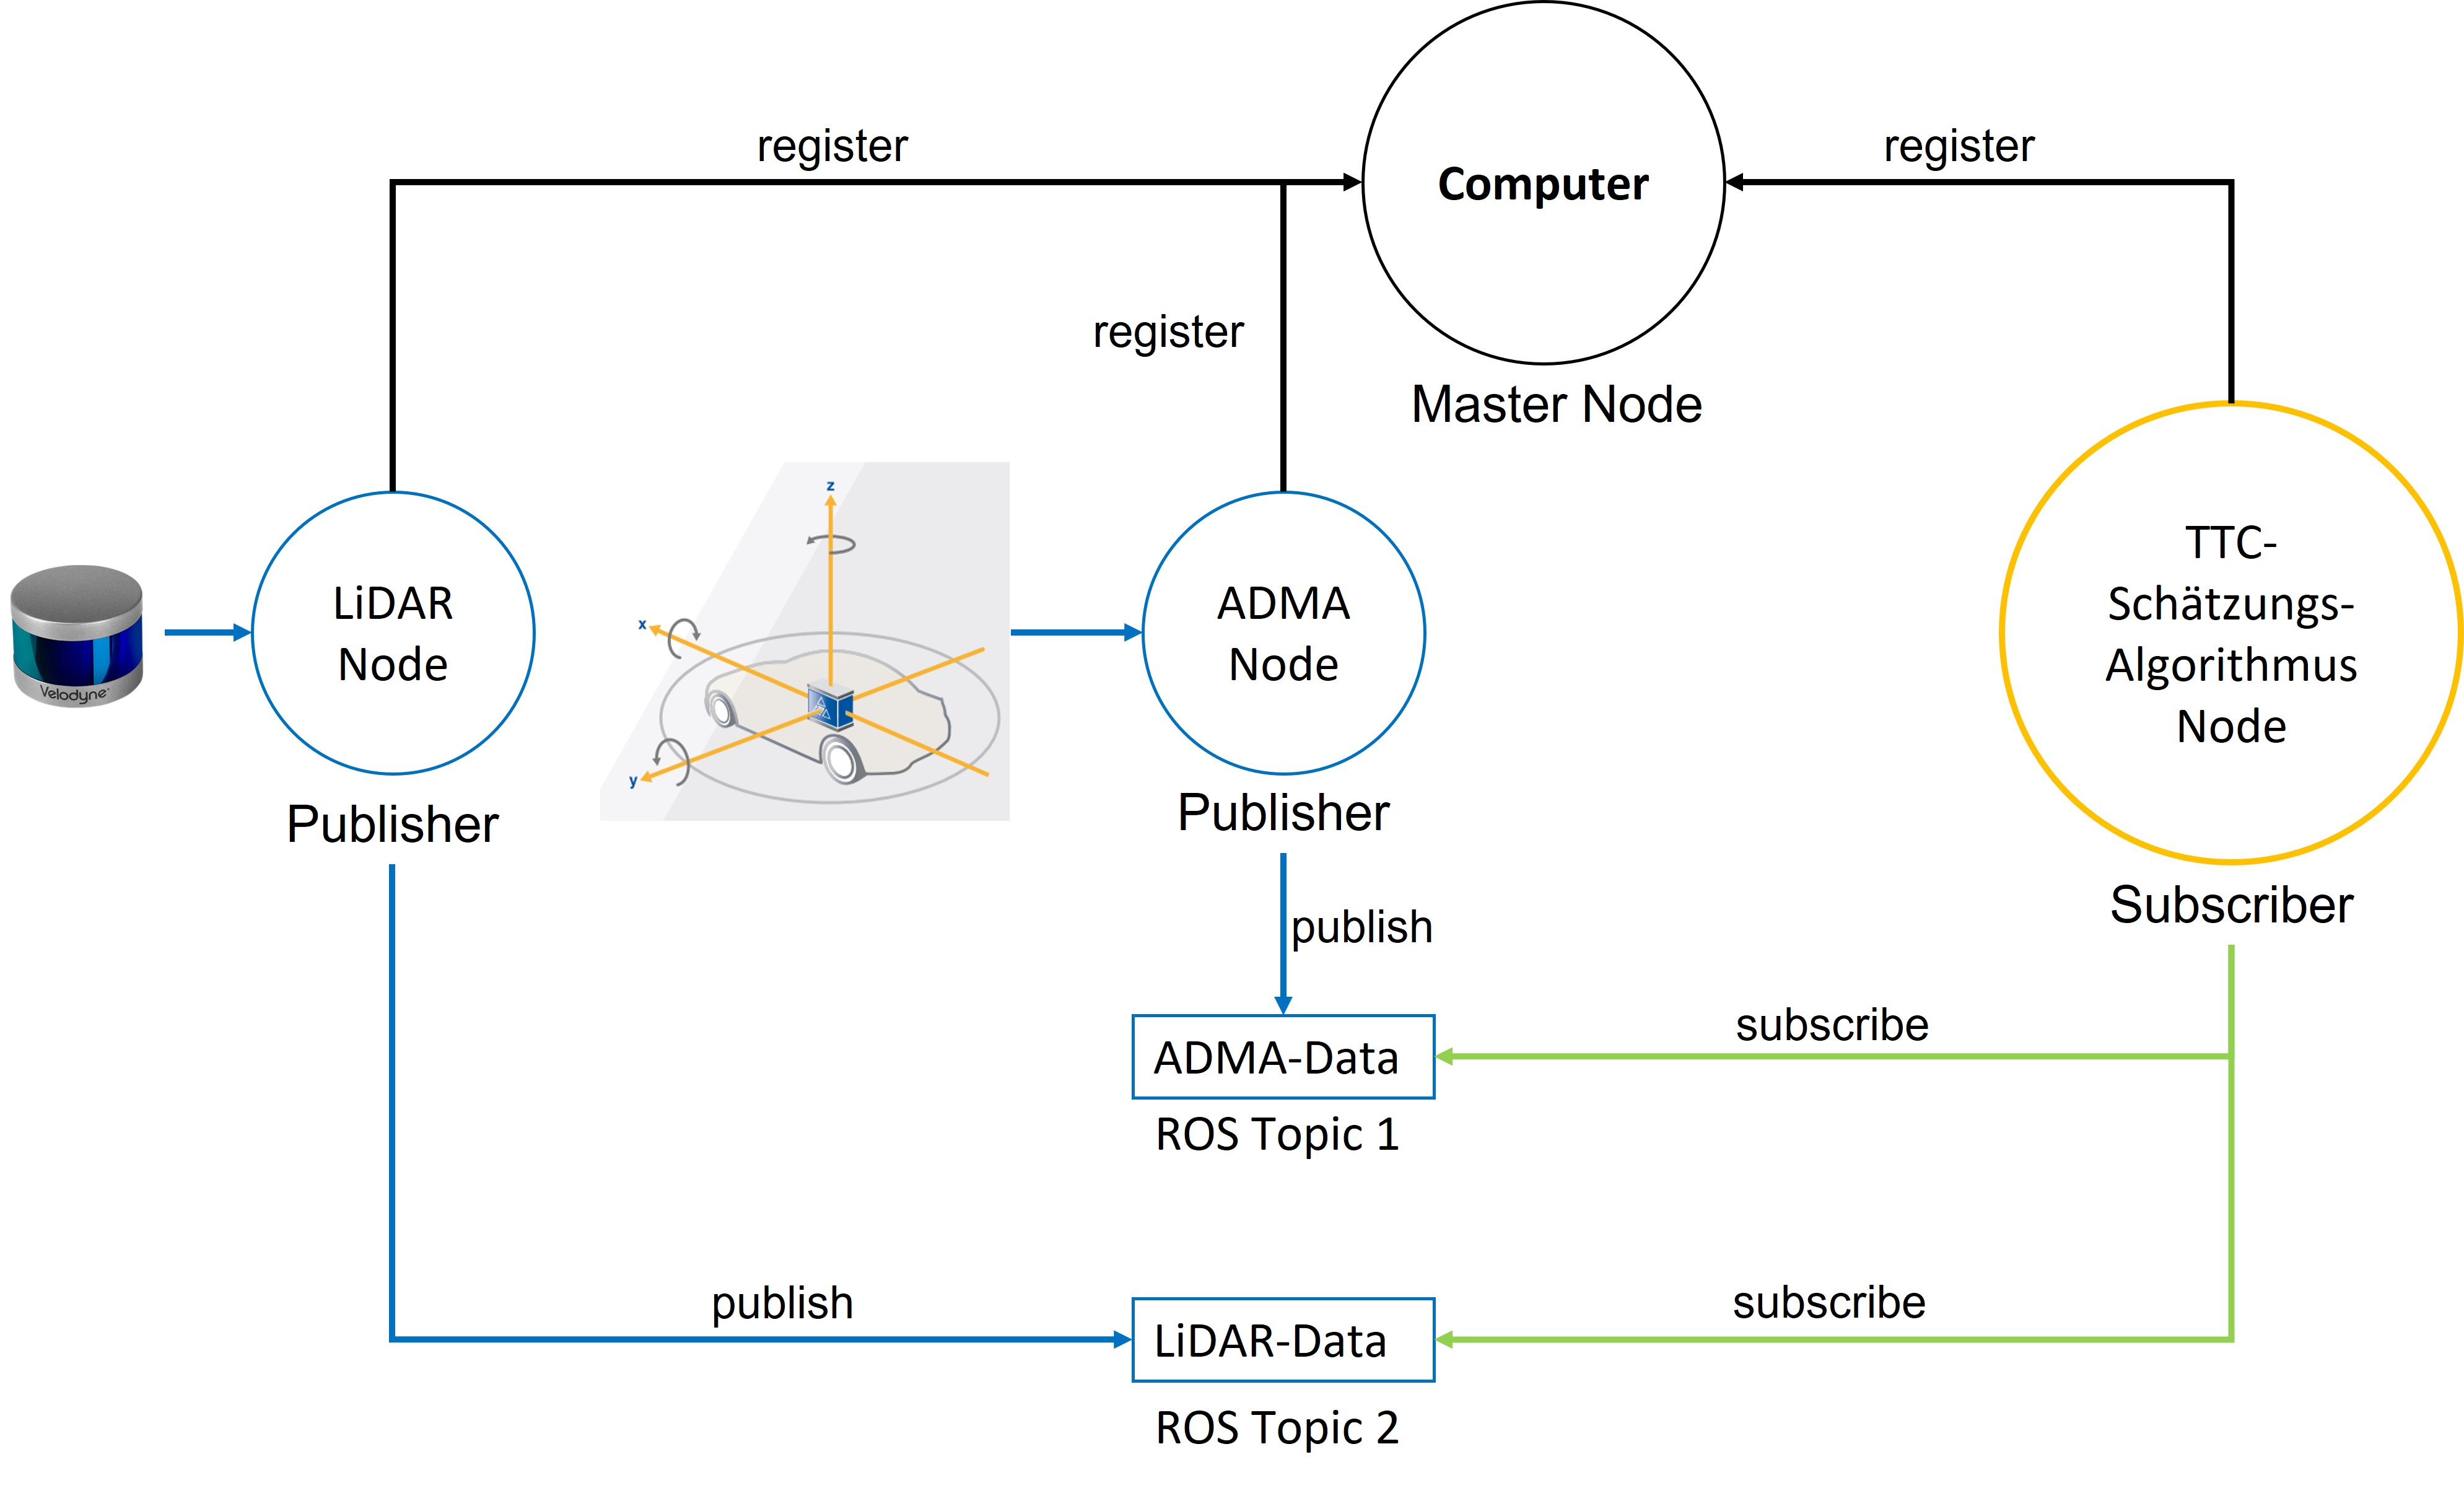
\includegraphics[scale=0.35]{required/ROS_Architecture.jpg}
%			\caption{Darstellung der ROS Architektur des Szenarios}
%		\end{figure}
%	\end{frame}
	\begin{frame}{Datenvorverarbeitung}{Region of Interest}
		\textbf{Motivation:} Reduzierung der zu verarbeitenden Sensordatenmenge.
		\begin{itemize}
			\item Je nach Anwendungsfall können nicht relevante Daten unberücksichtigt werden.
			\item Für unseren Anwendungsfall, nicht relevante Daten können durch die Verwendung von HD (engl. High Definition)-Karten herausgefiltert werden.
			\item HD-Karten liefern Informationen über die Straßeninfrastruktur.
			\item Durch den Einsatz eines ADMA ist der genaue Standort des Fahrzeugs bekannt.
			\item Folgerung: Feste Infrastrukturelemente (Gebäude, Masten, Ampeln) können ignoriert werden, wodurch sich die zu verarbeitende Datenmenge verringert.
		\end{itemize}
	\end{frame}

	\begin{frame}{Datenvorverarbeitung}{Region of Interest}
		\begin{figure}
			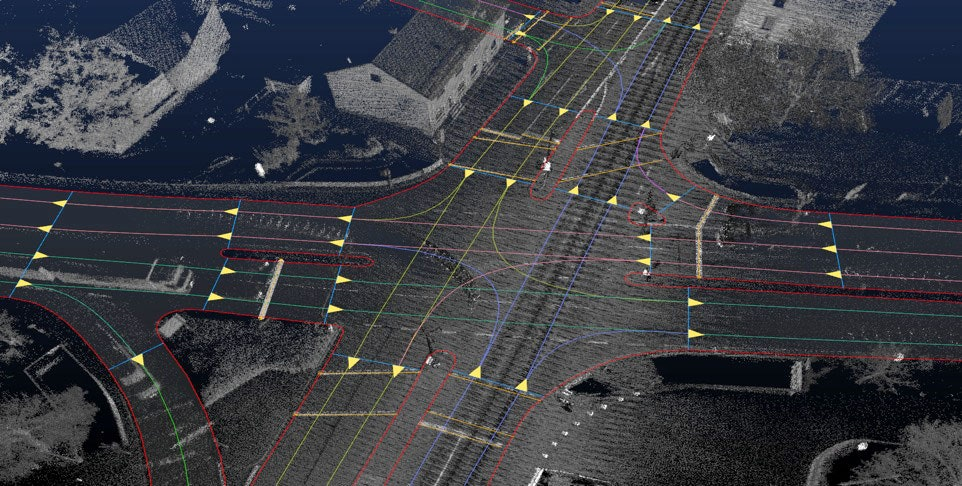
\includegraphics[scale=0.3]{required/HD-Map.jpg}
			\caption{Die Abbildung zeigt ein Beispiel für eine HD-Map. Die befahrbare Straße ist als farbige Linien dargestellt. [Miller.2022]}			
		\end{figure}
	\end{frame}
	\begin{frame}{Datenvorverarbeitung}{Region of Interest}
		Da die CARISSMA Teststrecke als HD-Karte vorliegt, kann man die LiDAR-Messungen außerhalb des befahrbaren Bereichs ignorieren.
		\begin{figure}
			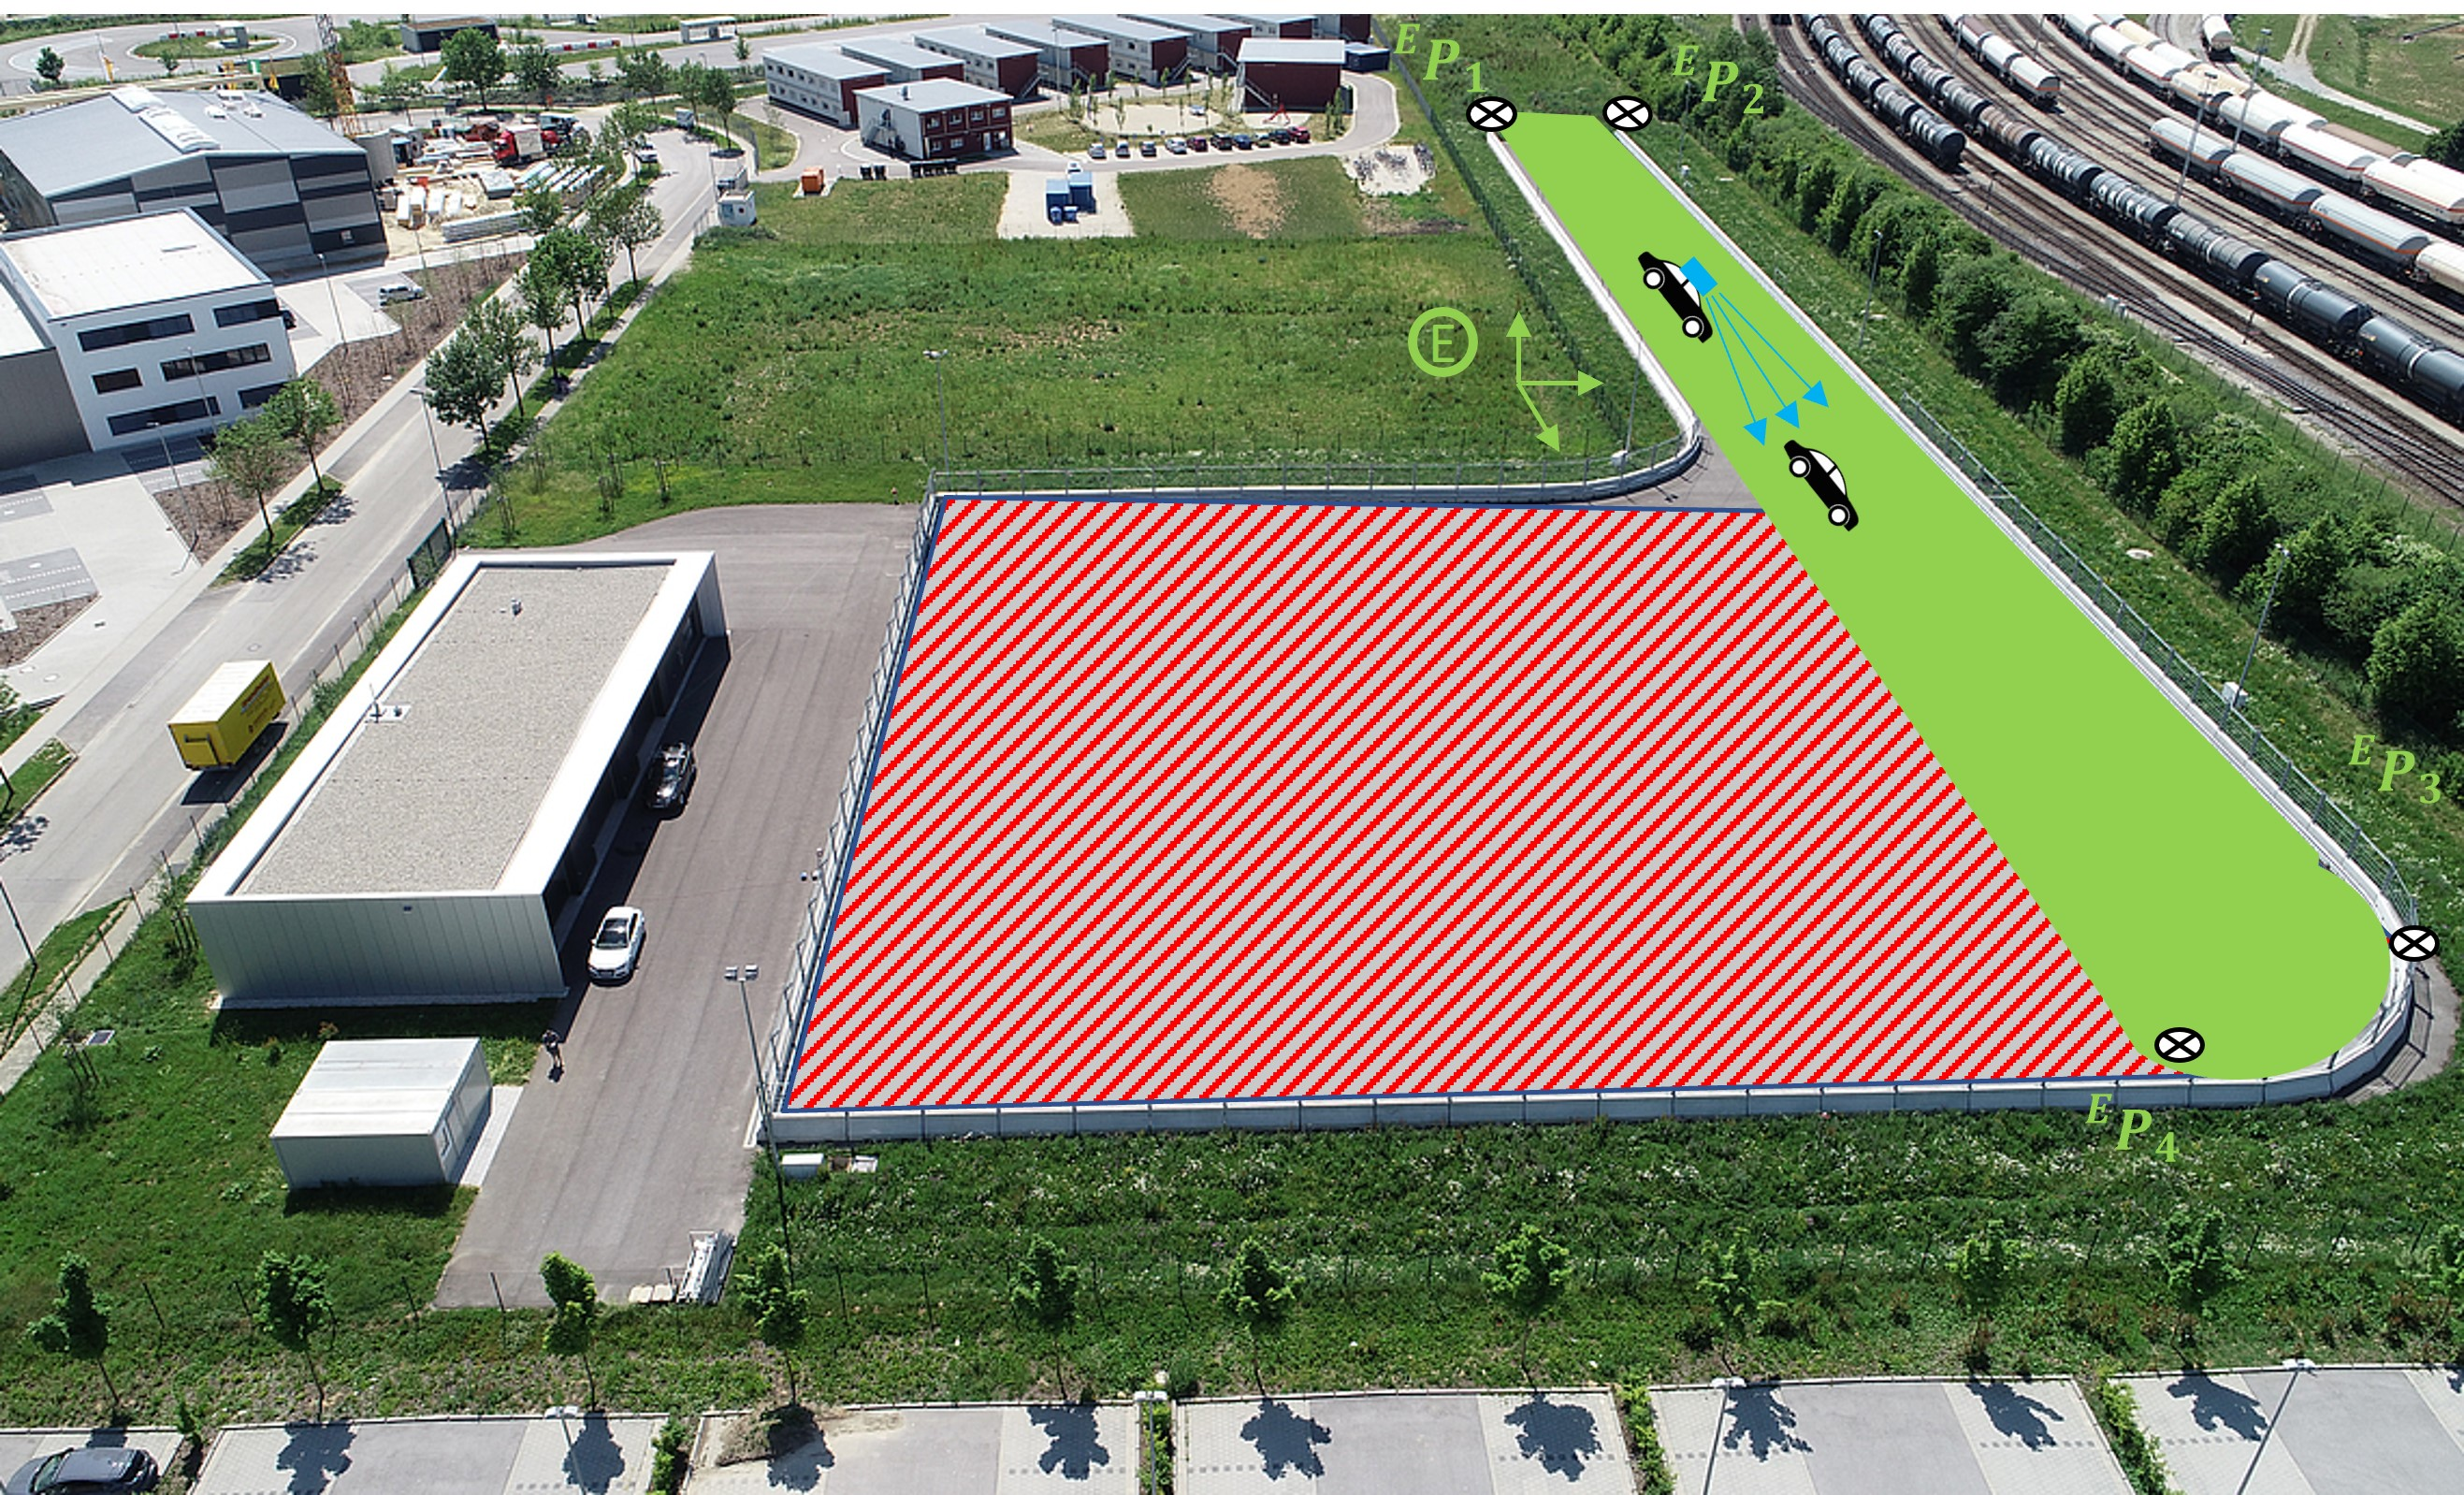
\includegraphics[scale=0.35]{required/ROI-Teststrecke.jpg}
			\caption{Die Abbildung zeigt die CARISSMA-Teststrecke. Mit \textcolor{green}{grün}, der befahrbare Bereich. Mit \textcolor{red}{rot}, der nicht befahrbare Bereich.}	
		\end{figure}
	\end{frame}
	\begin{frame}{Datenvorverarbeitung}{Region of Interest}
		Der befahrbare Bereich kann als ein Polygon definiert werden, das aus Eckpunkten besteht.\\
		Der $i$-th Eckpunkt kann definiert werden als
		\begin{align}
			\hspace*{0.2em}^E\vspace*{-0.2em}P_{i}=(x_i,y_i),
		\end{align}
wobei $(x_i,y_i)$ die $(x,y)$-Koordinaten des Eckpunktes im Global Frame sind.\\
		Wenn der befahrbare Bereich $\mathbf{P}$ aus 4 Eckpunkten besteht, kann er wie folgt definiert werden
		\begin{align}
			\mathbf{P}=\begin{matrix}
				\hspace*{0.2em}^E\vspace*{-0.2em}P_{1}&\hspace*{0.2em}^E\vspace*{-0.2em}P_{2}&\hspace*{0.2em}^E\vspace*{-0.2em}P_{3}&\hspace*{0.2em}^E\vspace*{-0.2em}P_{4}
			\end{matrix}
		\end{align}
	\textbf{Forschungsfrage:} Wenn die befahrbare Fläche bekannt ist, wie lassen sich dann nicht relevante LiDAR-Messungen herausfiltern? \textcolor{blue}{**s. inpolygon code**}
	\end{frame}
%\begin{frame}{Datenvorverarbeitung}{Region of Interest}
%		\begin{itemize}
%			\item Transformationsmatrizen: 
%		\end{itemize}
%		\textbf{Vorgehensweise:}
%		\begin{enumerate}
%			\item Transformation der LiDAR-Punkte $\hspace*{0.2em}^L\vspace*{-0.2em}P_{i}$ in das globale Koordinatensystem 
%			\item Filterung aller Punkte mit Koordinaten $(x,y)$ außerhalb des durch die 4 Punkte $\hspace*{0.2em}^E\vspace*{-0.2em}P_{i}$ aufgespannten Bereichs
%		\end{enumerate}
%	\end{frame}
	
	\begin{frame}{Datenvorverarbeitung}{Ground Subtraction}
		\footnotesize
		\textbf{Motivation:} Reduzierung der zu verarbeitenden Sensordatenmenge.
		\begin{itemize}
			\item LiDAR Sensor gibt zahlreiche Reflektionen der Fahrbahnoberfläche aus.
			\item Einige Forschungsarbeiten befassen sich mit der Aufgabe, Objekte aus dem Schatten auf dem Boden zu erkennen.\\
			\item Zur Vereinfachung wird in dieser Arbeit der Boden von der Punktwolke subtrahiert. 
			\item Folgerung: Verkleinerung des Lösungsraums.		
		\end{itemize}	
	\textbf{Forschungsfrage:} Wie kann man die Grundebene subtrahieren? 
		\begin{figure}
			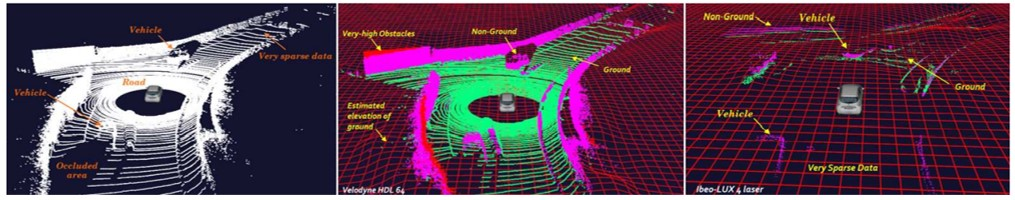
\includegraphics[scale=0.33]{required/Ground Subtraction.jpg}
			\caption{Die Abbildung zeigt ein Beispiel für eine Bodensubtraktion. Links: die rohe Punktwolke. In der Mitte die Punktwolkensegmentierung: bei Grün der Boden, bei Lila der Rest. Rechts: die Punktwolke ohne die Punkte, die dem Boden entsprechen. [Rummelhard.2017]}
        	\label{Ground Subtraction}
       	\end{figure}
	\end{frame}
	\begin{frame}{Datenvorverarbeitung}{Ground Subtraction}
		\begin{itemize}
			\item Zwei Optionen für die Subtraktion der Grundfläche sind: z-Filterung und der RANSAC-Algorithmus.
			\item Die z-Filterung bedeutet, dass alle Messungen unterhalb einer bestimmten Höhe weggelassen werden.
			\item Die Implementierung der z-Filterung ist schneller als die Implementierung des RANSAC-Algorithmus.
		\end{itemize}
	\textcolor{blue}{**s. z-th substraction code**}
		\begin{figure}
			
\includegraphics[scale=0.5]{required/Ground Subtraction Implementierung.jpg} 
			\caption{Die Abbildung zeigt eine grafische Darstellung der Bodensubtraktion. In Rot der Bereich, in dem die LiDAR-Messungen nicht berücksichtigt werden sollen. [Rummelhard.2017]}
		\end{figure}
	\end{frame}
	\begin{frame}{Datenvorverarbeitung}{Ground Subtraction}
		\footnotesize
		\begin{itemize}
			\item Der Ransac-Algorithmus ist robuster, insbesondere gegenüber Ausreißern, aber seine Implementierung ist zeitaufwendiger.		
			\item Der Algorithmus versucht, eine Ebenengleichung zu finden, die später als Schwellenwert für die Eliminierung von Punkten aus der Punktwolke verwendet wird.
			\item Es nimmt zufällige Punkte aus der Punktwolke, um die Grundflächengleichung zu finden. 
		\end{itemize}

		\begin{figure}
			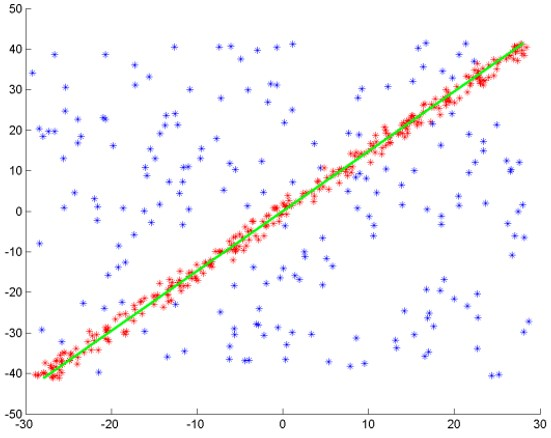
\includegraphics[scale=0.4]{required/RANSAC.jpg}
			\caption{Beispiel RANSAC-Algorithmus [RANSAC.2021]}
        	\label{Clustering}
		\end{figure}
	\end{frame}


\begin{frame}{KI-Methoden}{Ground Subtraction}
	\footnotesize		
	%		\textbf{Motivation:} Einfaches ML-Modell zur Prognose der TTC. Zudem eine gute Veranschaulichung des MLs.
	\begin{itemize}
		\item Annahme der Funktion $f(\textbf{x})$: Der Zielvektor \textbf{y} kann entsprechend der Rechenvorschrift
		\begin{equation}
			y = w^{\text{T}} x + t + \eta \text{ mit } \eta \backsim \mathcal{N}(0, \sigma^2) \text{,}
		\end{equation}
		\item[] wobei $w$ und $t$ Parameter sind, und $x$ die Dimension $N$ hat, abgebildet werden.		   
	\end{itemize}
	\begin{figure}
		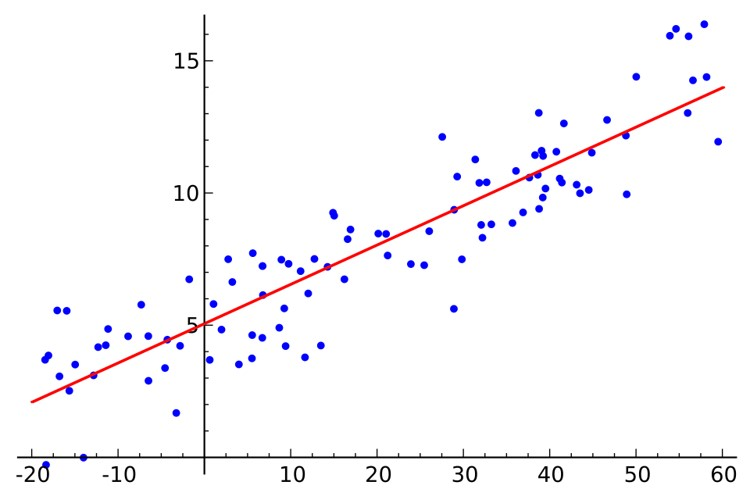
\includegraphics[scale=0.25]{required/Lineare_Regression.jpg}
		\caption{\scriptsize Lineare Basisfunktion [LinWik.2017]}
		\label{Over and Underfitting}
	\end{figure}
\end{frame}
\begin{frame}{KI-Methoden}{Ground Subtraction}
	\footnotesize
	\begin{itemize}			
		\item Für eine kompaktere Schreibweise lassen sich $w$ und $t$ in den Parametervektor $\Theta = [w^{\text{T}}, t]^{\text{T}}$ der Dimension $(N+1)$ zusammenfassen und der Eingang $x$ erweitern zu $ \tilde{x} = [x^{\text{T}}, 1]^{\text{T}}$.
		\item Damit gilt: $
		y = \Theta^{\text{T}} \tilde{x} + \eta \text{ mit } \eta \backsim \mathcal{N}(0, \sigma^2) \text{,} $
		\item Die Lösung für den gesuchten Parameter $\theta$ ergibt sich aus dem Minimum der Verlustfunktion. Für die quadratische Verlustfunktion bedeutet dies:
		\begin{equation}
			\theta = \underset{\theta}{\mathrm{argmin}} \left\{\ \frac{1}{M} \sum_{m=1}^M\ (y_m - \theta^{\text{T}} \tilde{x}_m)^2 \right\}\
		\end{equation}
		\item Die Ableitung der quadratischen Funktion hat eine Nullstelle im Minimum					\begin{equation}
			\frac{\delta}{\delta \theta^{\text{T}}} \Bigl( \frac{1}{M} \sum_{m=1}^M\ (y_m - \theta^{\text{T}} \tilde{x}_m)^2 \Bigr) 
			= \sum_{m=1}^M\ -(y_m - \theta^{\text{T}} \tilde{x}_m) \tilde{x}_m^{\text{T}}
			\stackrel{!}{=} 0 
		\end{equation}
		
	\end{itemize}
\end{frame}
\begin{frame}{KI-Methoden}{Ground Subtraction}
	Die Lösung ist:
	\begin{equation}
		\theta = \Bigl( \sum_{m=1}^M\ \tilde{x}_m \tilde{x}_m^{\text{T}} \Bigr)^{-1} \Bigl( \sum_{m=1}^M\ \tilde{x}_m y_m \Bigr)
	\end{equation}
	Schreibt man dieses Ergebnis in Matrix-Vektor-Notation, so werden alle Eingänge und Zielwerte aus dem Datensatz $\mathcal{D}$ in der Matrix $\tilde{X}$ und dem Vektor $y$ sortiert. 
	\begin{equation}
		\theta = ( \tilde{X}^{\text{T}} \tilde{X} )^{-1} \tilde{X}^{\text{T}} y
		\hspace{0.5 cm}	
		\text{, mit }			
		\tilde{X} = 
		\begin{bmatrix}
			\tilde{x}_1^{\text{T}} \\
			\tilde{x}_2^{\text{T}} \\	
			\vdots \\
			\tilde{x}_M^{\text{T}} \\		
		\end{bmatrix}
		\text{,  }
		y =	
		\begin{bmatrix}
			\tilde{y}_1 \\
			\tilde{y}_2 \\	
			\vdots \\
			\tilde{y}_M \\
		\end{bmatrix}						
	\end{equation}

\textcolor{blue}{**s. linear regression code**} \textcolor{blue}{**s. ransac code**}
\end{frame}

\begin{frame}{KI-Methoden}{Ground Subtraction}
	\small		
	\textbf{Motivation}
	\footnotesize
	\begin{itemize}
		\item Die Einschränkung durch Linearität ermöglicht es dem Algorithmus nicht die TTC fehlerfrei darzustellen.
		\item Ein klassischer Fall von Underfitting.
		\item Eine entscheidende Möglichkeit kompliziertere Zusammenhänge darzustellen, ist Nicht-Linearität in die Funktion zu bringen
		\item Eine Möglichkeit sind nicht-lineare Basisfunktionen. 
	\end{itemize}					
	\begin{figure}
		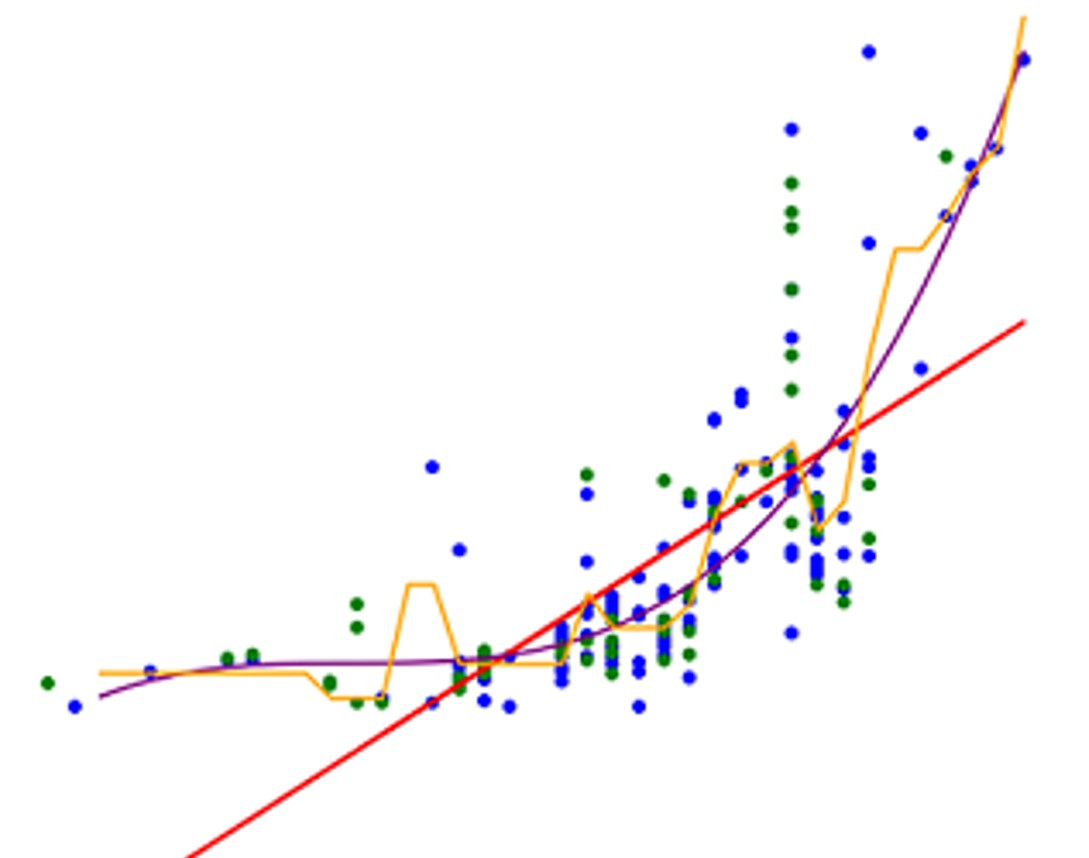
\includegraphics[scale=0.45]{required/Nicht_lineare_Regression.jpg}
		\caption{\scriptsize Verwendung von nicht-linearen Basisfunktionen [NlinWik.2017]}
		\label{Over and Underfitting}
	\end{figure}
\end{frame}
\begin{frame}{KI-Methoden}{Ground Subtraction}
	\begin{enumerate}
		\item Verwenden Sie die Datensätze der vorhergehenden Aufgabe.
		\item Analog zum beschriebenen Verfahren $x$ soll eine nichtlineare Basisfunktion $\varphi (x)$ verwendet werden. Folgende wird in diesem Fall gegeben:
		\begin{equation*}
			\varphi (x) = 
			\begin{bmatrix}
				\varphi_1(x) & \varphi_2(x) & \varphi_3(x) & \varphi_4(x) & \varphi_5(x) &
				\varphi_6(x) & \varphi_7(x) & \varphi_8(x) & \varphi_9(x)
			\end{bmatrix}
		\end{equation*}
		\item[] mit
		\begin{flalign}
			&\varphi_1 (x) = x_1, \hspace{0.2 cm} \varphi_2 (x) = x_2, \hspace{0.2 cm} 						\varphi_3 (x) = x_1^2, \hspace{0.2 cm} \varphi_4 (x) = x_2^2, \hspace{0.2 cm} 
			\varphi_5 (x) = x_1 x_2, \nonumber \\
			&\varphi_6 (x) = x_1^3,\hspace{0.2 cm} \varphi_7 (x) = x_2^3,\hspace{0.2 cm} \
			\varphi_8 (x) = x_1^2 x_2, \hspace{0.2 cm}  \varphi_9 (x) = x_1 x_2^2 \nonumber
		\end{flalign}
	\end{enumerate}
\end{frame}
%	\begin{frame}{KI-Methoden}{Implementierung: Nicht-lineare Basisfunktionen}
	%		\begin{enumerate}
		%			\setcounter{enumi}{2}	
		%			\item Bestimmung von $\theta$ für das neue Regressionsmodell. Test der Ausgabe $\hat{y}$ für den Testdatensatz $\mathcal{D}_\text{test}$.
		%			\item Visualisierung des Zusammenhangs von $d$ und $v_x,rel$ zu $\hat{y}$ für das berechnete Regressionsmodell. Visualisierung des Datensatzes $\mathcal{D}_\text{test}$ im selben Plot.
		%			\item Integration in die ROS-Pipeline zur Bestimmung der Kritikalität TTC online
		%			\item Zusatzaufgabe: Untersuchen sie die Folgen einer Änderung des Trainingsdatensatzes oder der Basisfunktion
		%		\end{enumerate}
	%	\end{frame}
\begin{frame}{KI-Methoden}{Ground Subtraction}
	\begin{itemize}
		\item Basiert auf der linearen Regression, wobei $x$ durch $\phi (x)$ ersetzt wird.
		\begin{equation}
			y = w^{\text{T}} \varphi (x) + t + \eta
			\hspace{0.2 cm}
			\text{mit}
			\hspace{0.2 cm}
			\eta \backsim \mathcal{N}(0, \sigma^2)
			\hspace{0.2 cm}
			\text{und} \hspace{0.2 cm} 			
			\varphi (x) = [ \varphi_1 (x), \varphi_2 (x), \dots, \varphi_H (x)]^{\text{T}} \text{,}
		\end{equation}
		\item[] wobei die Funktionen $\varphi (x)$ nichtlinear sein können
		\item Analog zur vorherigen Herleitung ergibt sich:
		\begin{equation}
			\tilde{\varphi} (x_m)= 
			\begin{bmatrix}
				\varphi (x_m)^{\text{T}} & 1
			\end{bmatrix}^{\text{T}}
		\end{equation}
		\begin{equation}
			\theta = \Bigl( \sum_{m=1}^M\ \tilde{\varphi} (x_m) \tilde{\varphi} (x_m)^{\text{T}} \Bigr)^{-1} \Bigl( \sum_{m=1}^M\ \tilde{\varphi} (x_m) y_m \Bigr) 
		\end{equation}
	\end{itemize}
\end{frame}
\begin{frame}{KI-Methoden}{Ground Subtraction}
	\begin{itemize}
		\item In Matrixschreibweise ergibt sich:			
		\begin{equation}
			\theta = \Bigl( \tilde{\phi}^{\text{T}} \tilde{\phi} \Bigr) ^{-1} \tilde{\phi}^{\text{T}} y
		\end{equation}
		\item[] mit
		\begin{equation}
			\tilde{\phi} =
			\begin{bmatrix}
				\tilde{\varphi} (x_1)^{\text{T}} \\
				\tilde{\varphi} (x_2)^{\text{T}} \\
				\vdots \\
				\tilde{\varphi} (x_M)^{\text{T}} \\			
			\end{bmatrix}
			\text{,}
			\hspace{0.2 cm}
			y = 
			\begin{bmatrix}
				y_1 \\
				y_2 \\
				\vdots \\
				y_M
			\end{bmatrix}
		\end{equation}
	\end{itemize}	

\end{frame}	




	\begin{frame}{Datenvorverarbeitung}{Clustering}
		\small
		\textbf{Motivation:} um eine Objektliste aus der Punktwolke zu erstellen. 
		\begin{itemize}
			\item Verwendung der \enquote{Ähnlichkeit} von Datenpunkten, um zusammengehörende Punkte zu erkennen und zu segmentieren.
%			\item Ziel ist, die Struktur der Eingangsdaten zu lernen und eine automatische Segmentierung in Gruppen ähnlicher Datenpunkte vorzunehmen
		\end{itemize}
		\textbf{Forschungsfrage:} Welche Features können zum Clustern von Punkten verwendet werden? 
		\begin{figure}
			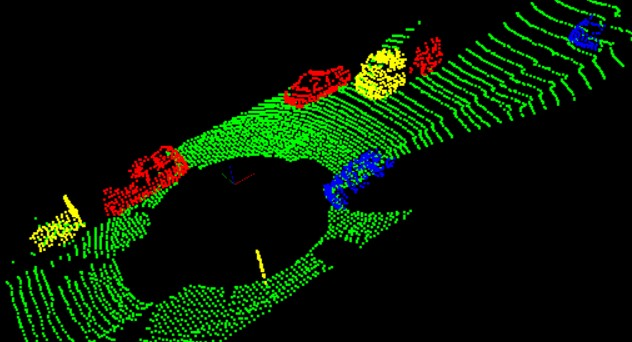
\includegraphics[scale=0.37]{required/Clustering.jpg}
			\caption{Die Abbildung zeigt ein Beispiel für Clustering. Mit grün, die Grundplatte. Bei rot, blau und gelb, die Fahrzeuge. [Hyin.2018]}
        	\label{Clustering}
		\end{figure}
	\end{frame}
	\begin{frame}{Datenvorverarbeitung}{Clustering}
		\begin{itemize}
\item Für unseren Anwendungsfall, bei dem die Grundfläche weg ist und sich nur wenige Objekte in der Umgebung befinden, kann eine Distanz-Clustering vorgenommen werden.\\
\item Auf Basis des $k$-Means Clusteralgorithmus sollen die Datenpunkte des vorausfahrenden Autos gruppiert und segmentiert werden.
		\end{itemize}
	\end{frame}		
	\begin{frame}{Datenvorverarbeitung}{Clustering}
		\textbf{Allgemein:}
		\begin{itemize}
			\item Mehrere Optionen bei der Art der durchgeführten Clusteranalyse: partionierende, modellbasierte, hierachische, wahrscheinlichkeitsdichtebasierte, gitterbasierte Verfahren und Spectral Clustering
			\item In unserem Fall ($k$-Means Clustering): partionierendes Cluster-Verfahren, bei dem auf Basis der Merkmale der Datenpunkte ein Clustering vorgenommen wird. Jeder Punkt  $v_m$ des Datensatzes $\mathcal{D}$ wird eindeutig einem Cluster $C_1, ..., C_k$ zugewiesen. Das Cluster $C_K$ kann dementsprechend als Partion des Eingangsraums $\mathbb{R}^N$ interpretiert werden.
			\begin{equation}
				\mathcal{D} = \{v_1, ..., v_M \}
			\end{equation}
	\end{itemize}
	\end{frame}
	\begin{frame}{Datenvorverarbeitung}{Clustering}
		\textbf{Beschreibung:} Aus einer Menge von ähnlichen Objekten wird eine vorher bekannte Anzahl von $k$ Clustern gebildet. Die Aufgabe wird gelöst, indem jeweils ein Repräsentant $c_k$ für jedes Cluster $C_k$ gesucht wird und zwar derart, dass alle Datenpunkte aus $\mathcal{D}$ nahe an ihrem jeweiligen Repräsentanten sind. \\
		\textbf{Umsetzung:} 
		\begin{itemize}
			\item Wenn $d(v_m, c_k)$ eine Distanz zwischen Eingangspunkt $v_m$ und Repräsentant des Clusters $c_k$ darstellt, so lässt sich die zu lösende Optimierungsaufgabe schreiben als
			\begin{equation}
				\{c_1, ..., c_k\}  = \underset{\{c_1',...,c_k'\}}{\mathrm{argmin}} \left\{\ \sum_{m=1}^M\ \underset{k=1, ...,K}{\mathrm{min}} d(v_m, c_k') \right\}\
			\end{equation}
			\item Diese Optimierungsaufgabe ist nicht konvex.
		\end{itemize}
 	\end{frame}
 	\begin{frame}{Datenvorverarbeitung}{Clustering}
 		\begin{itemize}
 			\item Um die nicht konvexe Optimierungsaufgabe zu lösen wird ein iteratives Verfahren, der $k$-Means Algorithmus verwendet. Dieser findet ein lokales Optimum.
 			\item Nutzt man im $k$-Means Algorithmus als Distanzmaß die quadrierte Euklidische Distanz
 			\begin{equation}
 			 	d(v_m, c_k) = \lVert v_m - c_k \rVert_2 ^2
 			\end{equation}
 			\item Wird die Optimierungsaufgabe zu einer Minimierung der quadratischen Abweichungen von den Cluster-Schwerpunkten der Cluster $S_i$. Es kann von Clustering durch Varianzminimierung gesprochen werden. \textcolor{blue}{**s. k-means code**}
 			\begin{equation}
				J = \sum_{i=1}^k\ \sum_{x_j \in S_i}^{}\ \lVert v_m - c_k \rVert_2^2
			\end{equation}
 		\end{itemize}
 	\end{frame}
%	\begin{frame}{Datenvorverarbeitung}{Clustering}
%		\textbf{Umsetzung LIoyd-Algorithmus:}
%		\begin{itemize}
%			\item 
%			\begin{enumerate}
%				\item Initialisierung: Wähle k zufällige Mittelwerte (Means): $m_1^{1},...,m_k^{1}$ aus dem Datensatz
%				\item Zuordnung: Jedes Datenobjekt wird dem Cluster zugeordnet, bei dem die Cluster-Varianz am wenigsten erhöht wird
%				\begin{equation}
%					S_i^{t} = { x_j : \lVert x_j - m_i^{t} \rVert ^2 \text{ für alle } i^{*}=1, ..., k}
%				\end{equation}
%				\item Aktualisierung: Neuberechnung der Mittelpunkte der Cluster:
%				\begin{equation}
%					m_i^{t+1} = \frac{1}{|S_i^{(t)}|} \sum_{x_j \in S_i}^{}\ x_j
%				\end{equation}
%				\item Schritte 2-3 werden wiederholt, bis die Zentren $c_1, ..., c_k$ stabil sind, d. h. sich nicht mehr signifikant ändern.
%			\end{enumerate}
%
%		\end{itemize}
%	\end{frame}
%	\begin{frame}{Datenvorverarbeitung}{Clustering}
%		\textbf{Vorteil:} 
%		\begin{itemize}
%			\item Leistungsfähigkeit (Komplexität $\mathcal{O}(kM)$ pro Iteration)
%			\item Einfache Umsetzung, die lokales Minimum für die Optimierungsaufgabe liefert
%			\item Eines der am häufigsten verwendeten Datensätze
%		\end{itemize} 		
%		\textbf{Nachteile:}		
%		\begin{itemize}
%			\item Gefundene Lösung hängt stark von der initialen, zufälligen Startpunkten ab
%			\item Ausreißer in den Daten aus $\mathcal{D}$ beeinflussen , aufgrund der Mittelwertbildung für die Bestimmung der Clusterzentren, das finale Ergebnis stark
%			\item Anzahl der Clusterzentren $k$ bereits im Voraus gewählt
%		\end{itemize}
%	\end{frame}
	\begin{frame}{Datenvorverarbeitung}{Objektliste}
		\footnotesize
	\textbf{Motivation:} Um die Kritikalität mit Hilfe von KI-Algorithmen abschätzen zu können, wird eine Objektliste benötigt. Die Objektliste enthält Informationen über die Objekte in der Umgebung: Position, Geschwindigkeit, Ausrichtung usw.\\
	Ein Bounding Box kann helfen, die Objekte in der Umgebung zu visualisieren, da er ihre Ausrichtung, Breite, Länge und Höhe anzeigt. Es hilft auch bei der Visualisierung der Clustering-Leistung.
	
	\textcolor{blue}{**s. bounding box code**}
%			\item \textbf{Vorgehen:} Bestimmung der Objektgrenzen auf Basis der segmentierten Objekt-LiDAR Punkte. Deren Koordinaten können für eine Bestimmung der Objektposition verwendet werden.
%			\item \textbf{Implementierungshinweise:} Verwenden sie zur Vereinfachung den 2D Bird's eye view. Bestimmen Sie auf Basis der Punktkoordinaten das Objektzentrum und schätzen sie mit ihrem Wissen über die typische Größe eines Autos die bounding box. Mögliche Größe: $1.6 \text{ m} \times 3.9 \text{ m}$.
		\begin{figure}
			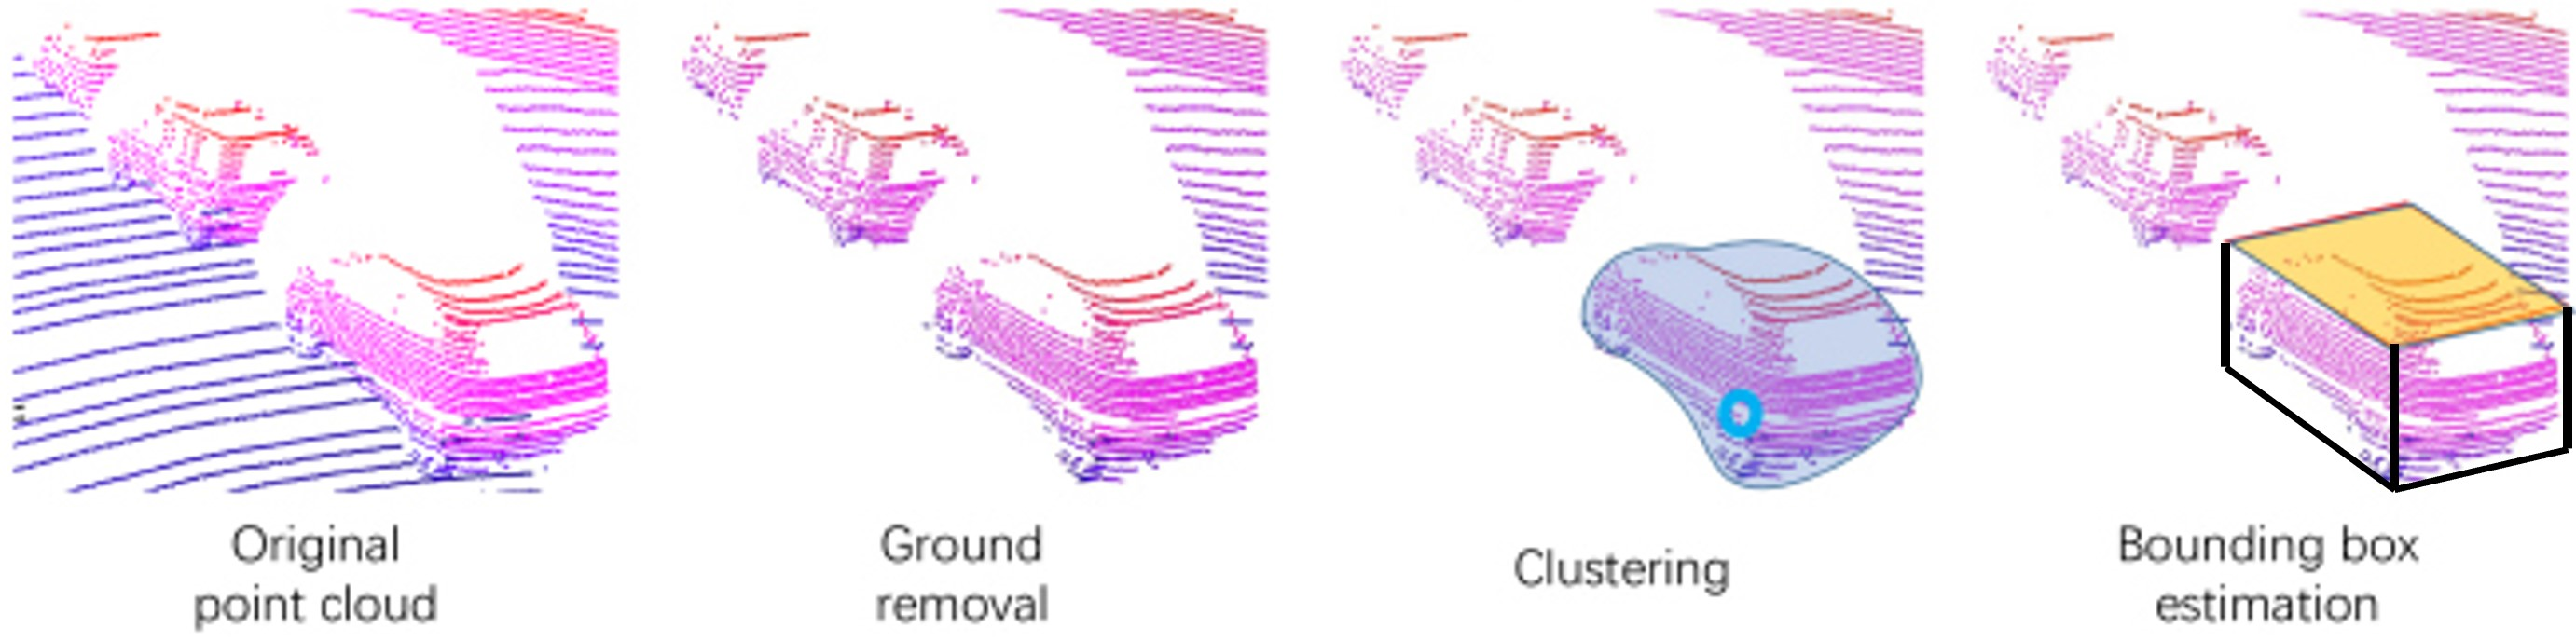
\includegraphics[scale=0.4]{required/Bounding_Box.jpg}
			\caption{Veranschaulichung der Bounding Box Bestimmung. Modifiziert von [Wang.2019]}
        	\label{Ground Subtraction}
       	\end{figure}
	\end{frame}
%	\begin{frame}{KI-Methoden}{Grundlagen der künstlichen Intelligenz}
%		Im Folgenden wird ein kurzer Einstieg in das Thema künstlichen Intelligenz vermittelt. Der Fokus liegt auf einem oberflächlichen Verständnis für Begrifflichkeiten und Methoden. Es sei jedoch erwähnt, dass künstlichen Intelligenz Mathematik und Statistik basiert, welche für ein tieferes Verständnis nötig ist, aber den Rahmen dieses Projektes übertreffen würde.
%		Für einen tieferen Einstieg empfiehlt sich bspw.: 
%		\begin{itemize}
%			\item  Literatur: z.B. [Botsch.2020]
%			\item Diverse Online-Quellen und Videos
%			\item Studium im entsprechenden Bereich 
%		\end{itemize}
%	\end{frame}
	\begin{frame}{KI-Methoden}{Grundlagen der künstlichen Intelligenz}
		\footnotesize
		Der Begriff künstlichen Intelligenz fasst Methoden der Signalverarbeitung zusammen, die statistische Zusammenhänge in Daten mit Hilfe von Computern finden und damit in der Lage sind, zukünftige Daten vorherzusagen.\\ Man spricht auch von der künstlichen Generierung von Wissen aus Erfahrung. Das maschinelle Lernen beruht auf der mathematischen Statistik und beschäftigt sich mit dem „Lernen“ aus Daten, d. h. mit dem Finden von Gesetzmäßigkeiten in den Daten.\\
		\begin{figure}
			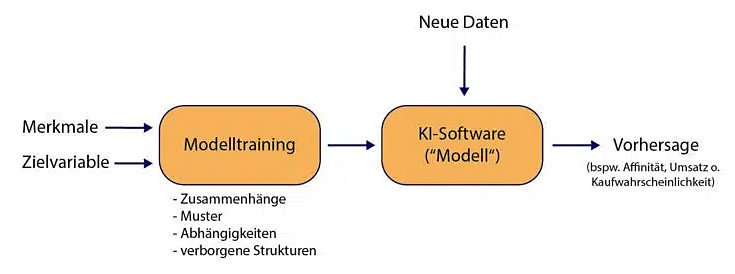
\includegraphics[scale=0.45]{required/ML_Einfuhrung.jpg}
			\caption{Grundkonzept des maschinellen Lernens [Wuttke.2020]}
        	\label{Ground Subtraction}
       	\end{figure}

	\end{frame}
	\begin{frame}{KI-Methoden}{Grundlagen der künstlichen Intelligenz}
		künstlichen Intelligenz ist ...
		\begin{itemize}
%			\item ein Teilbereich der künstlichen Intelligenz
			\item zunehmend relevant in allen Ingenieurswissenschaften, da die Rechenleistung und verfügbare Datenmenge in den letzten Jahren stark zugenommen hat.
			\item fähig zahlreiche komplexe praktische Anwendungen erfolgreich zu bearbeiten.
	\end{itemize}		
		Die Arbeitsschritte lassen sich grob folgender Maßen zusammenfassen:
		\begin{enumerate}
			\item Definition der Ziele.
			\item Vorbereitung der Daten.
			\item Lernphase.
			\item Interpretation der Ergebnisse.
			\item Nutzung in einer praktischen Anwendung.
		\end{enumerate}
	\end{frame}
    \begin{frame}{KI-Methoden}{Grundlagen der künstlichen Intelligenz}
		\begin{figure}
			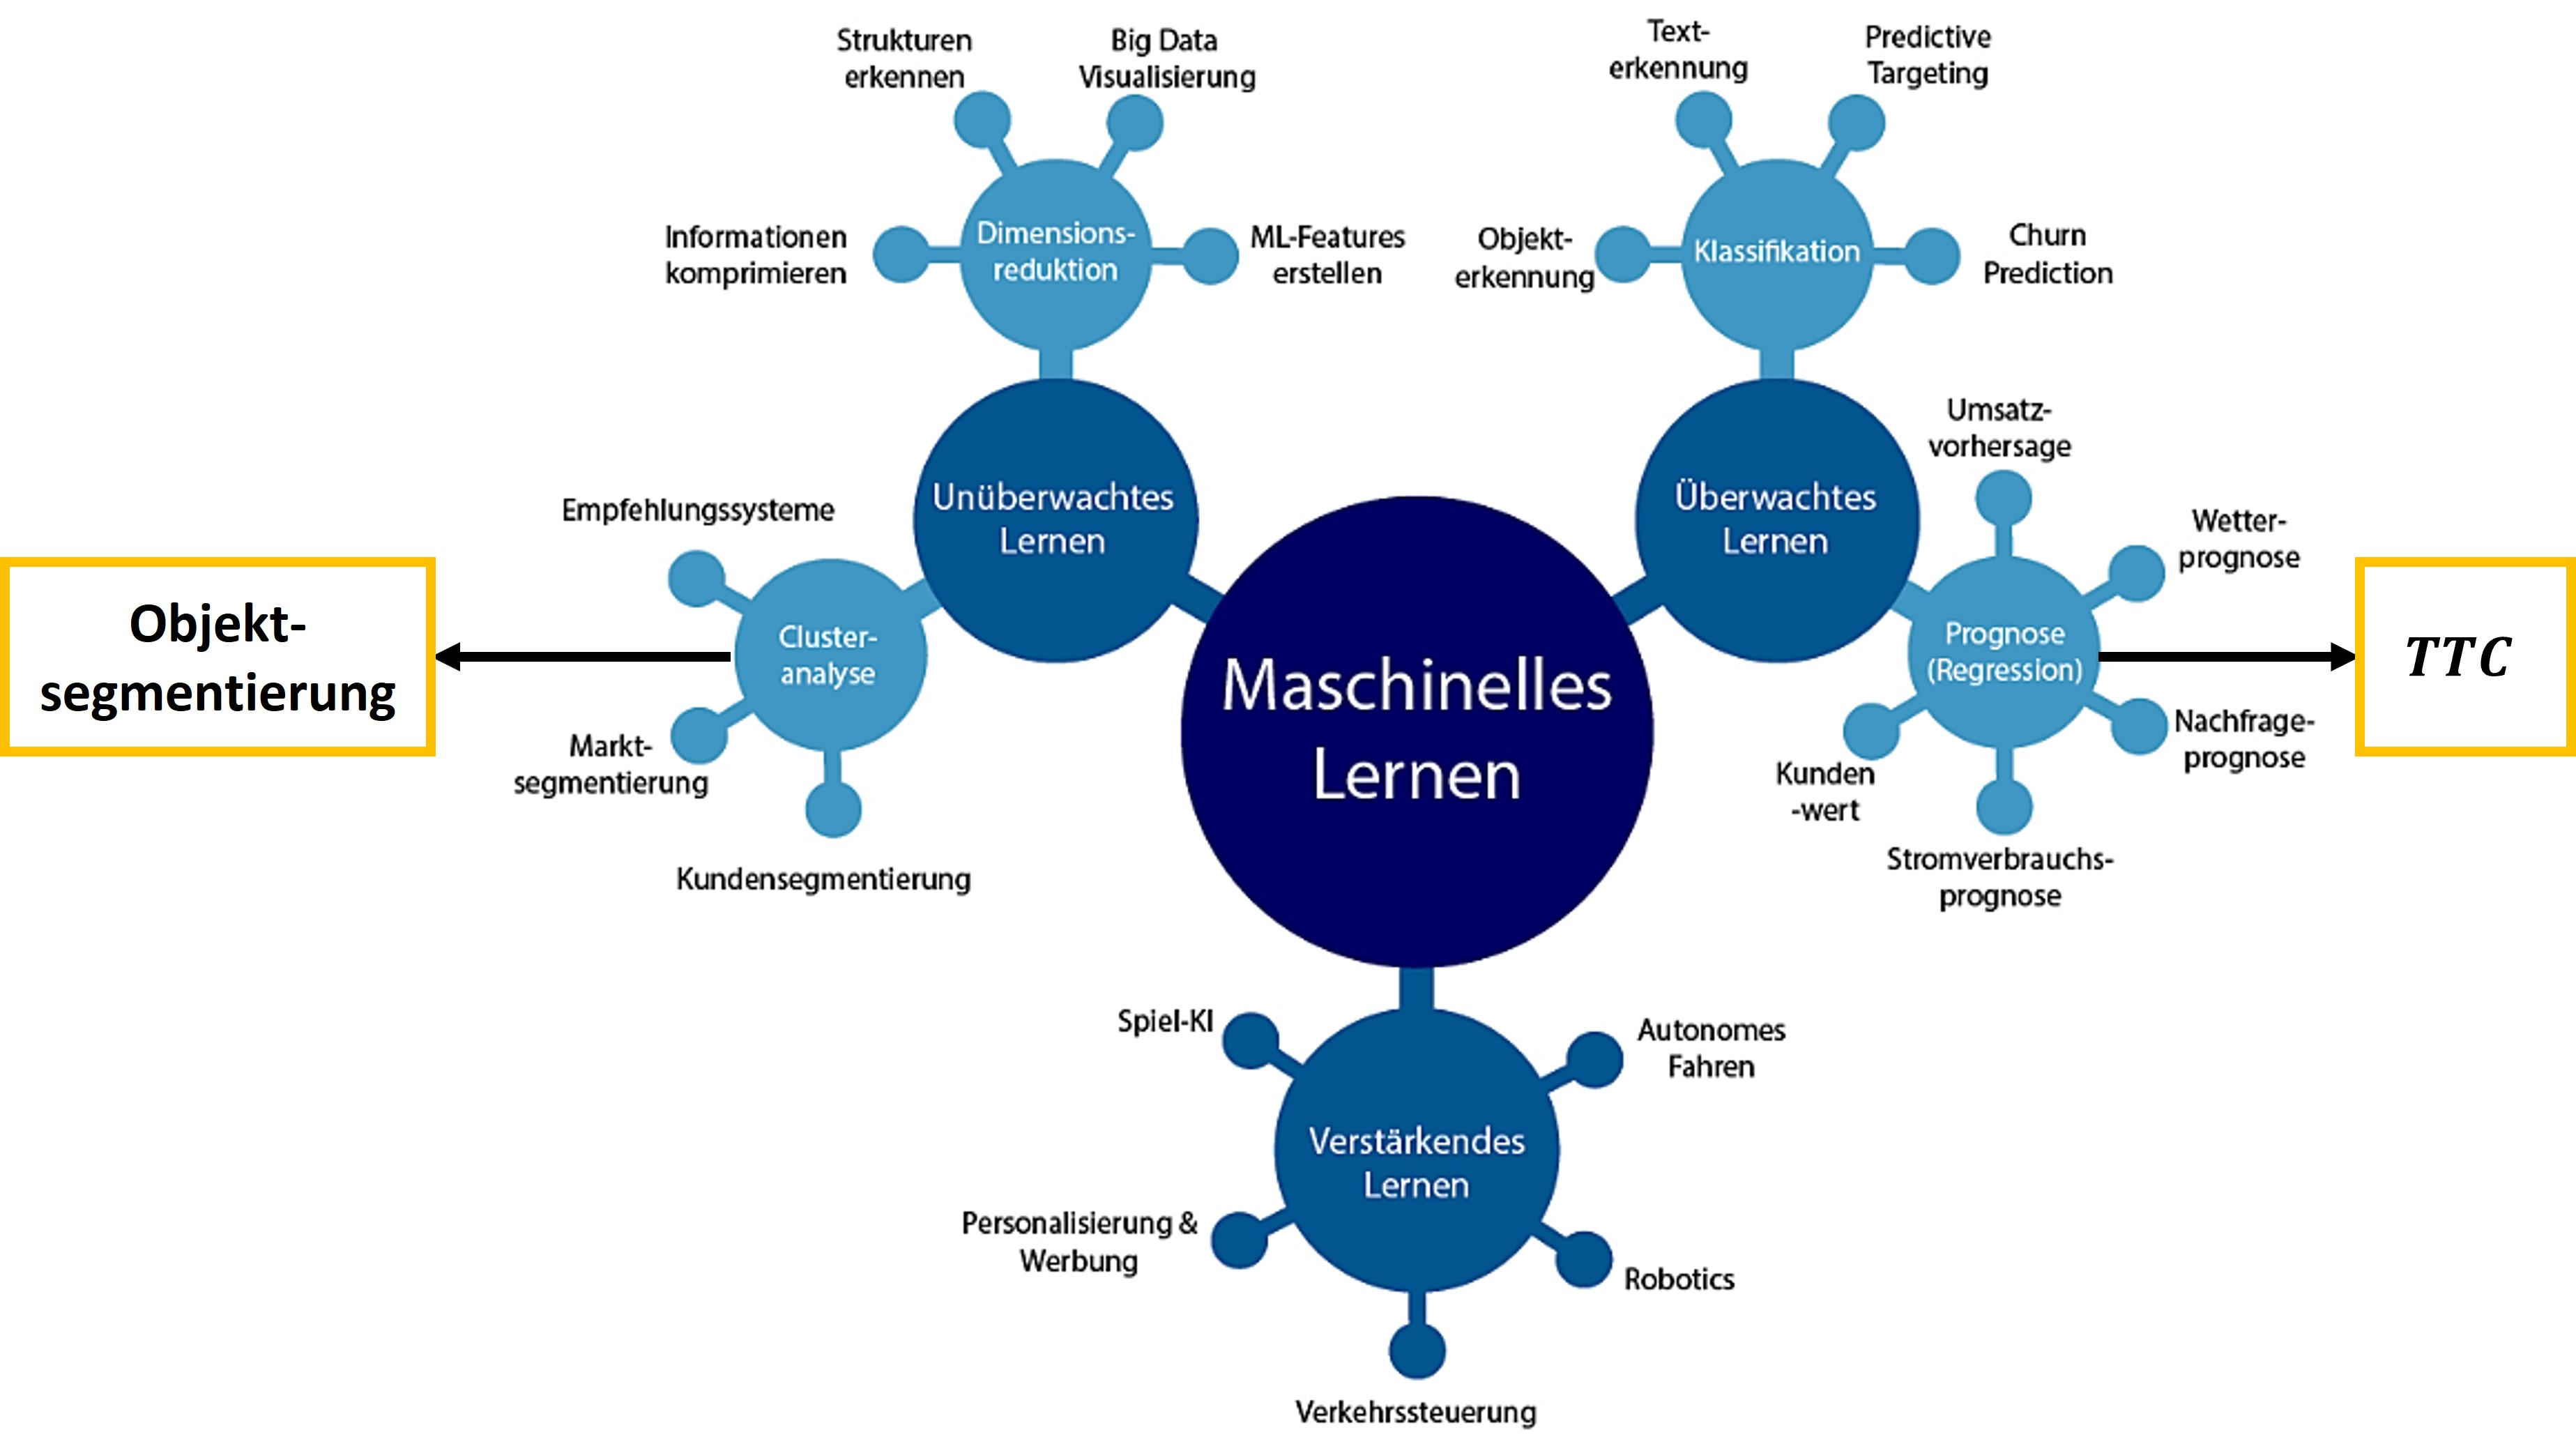
\includegraphics[scale=0.4]{required/Bereiche_Machine_Learning.jpg}
			\caption{Anwendungsgebiete des maschinellen Lernens[Wuttke.2020]}
        	\label{Ground Subtraction}
       	\end{figure}
     
    \end{frame}
    \begin{frame}{KI-Methoden}{Grundlagen der künstlichen Intelligenz}
		\vspace{1cm}       	
       	\textbf{Hinweis:} Der bereits angewandte $k$-Means-Algorithmus entspricht damit Maschinellem Lernen. Die Art wird des unüberwachten Lernens (eng. Unsupervised Learning) genannt. Bei dieser lernt Algorithmus allein aus den Eingängen, es gibt keine zugehörigen Labels. Ziel ist es, die Struktur in den Eingangsdaten zu lernen und ein Modell dafür zu erstellen.
	\end{frame}
	\begin{frame}{KI-Methoden}{Grundlagen der künstlichen Intelligenz}
		\small	
		\textbf{Überwachtes Lernen} (engl. Supervised Learning)	
		\footnotesize
		\begin{itemize}
			\item Eine Art des maschinellen Lernens (Andere: Unsupervised Learning, Semi-Supervised Learning, Reinforcement Learning)
			\item Ein Algorithmus lernt aus Beispielen von gelabelt Eingängen, d. h. es sind Eingangsdaten und zugehörige Labels
für das Lernen vorhanden. Ziel ist es, Vorhersagen für neue, unbekannte Eingangsdaten zu machen.
		\end{itemize}
		\begin{figure}
			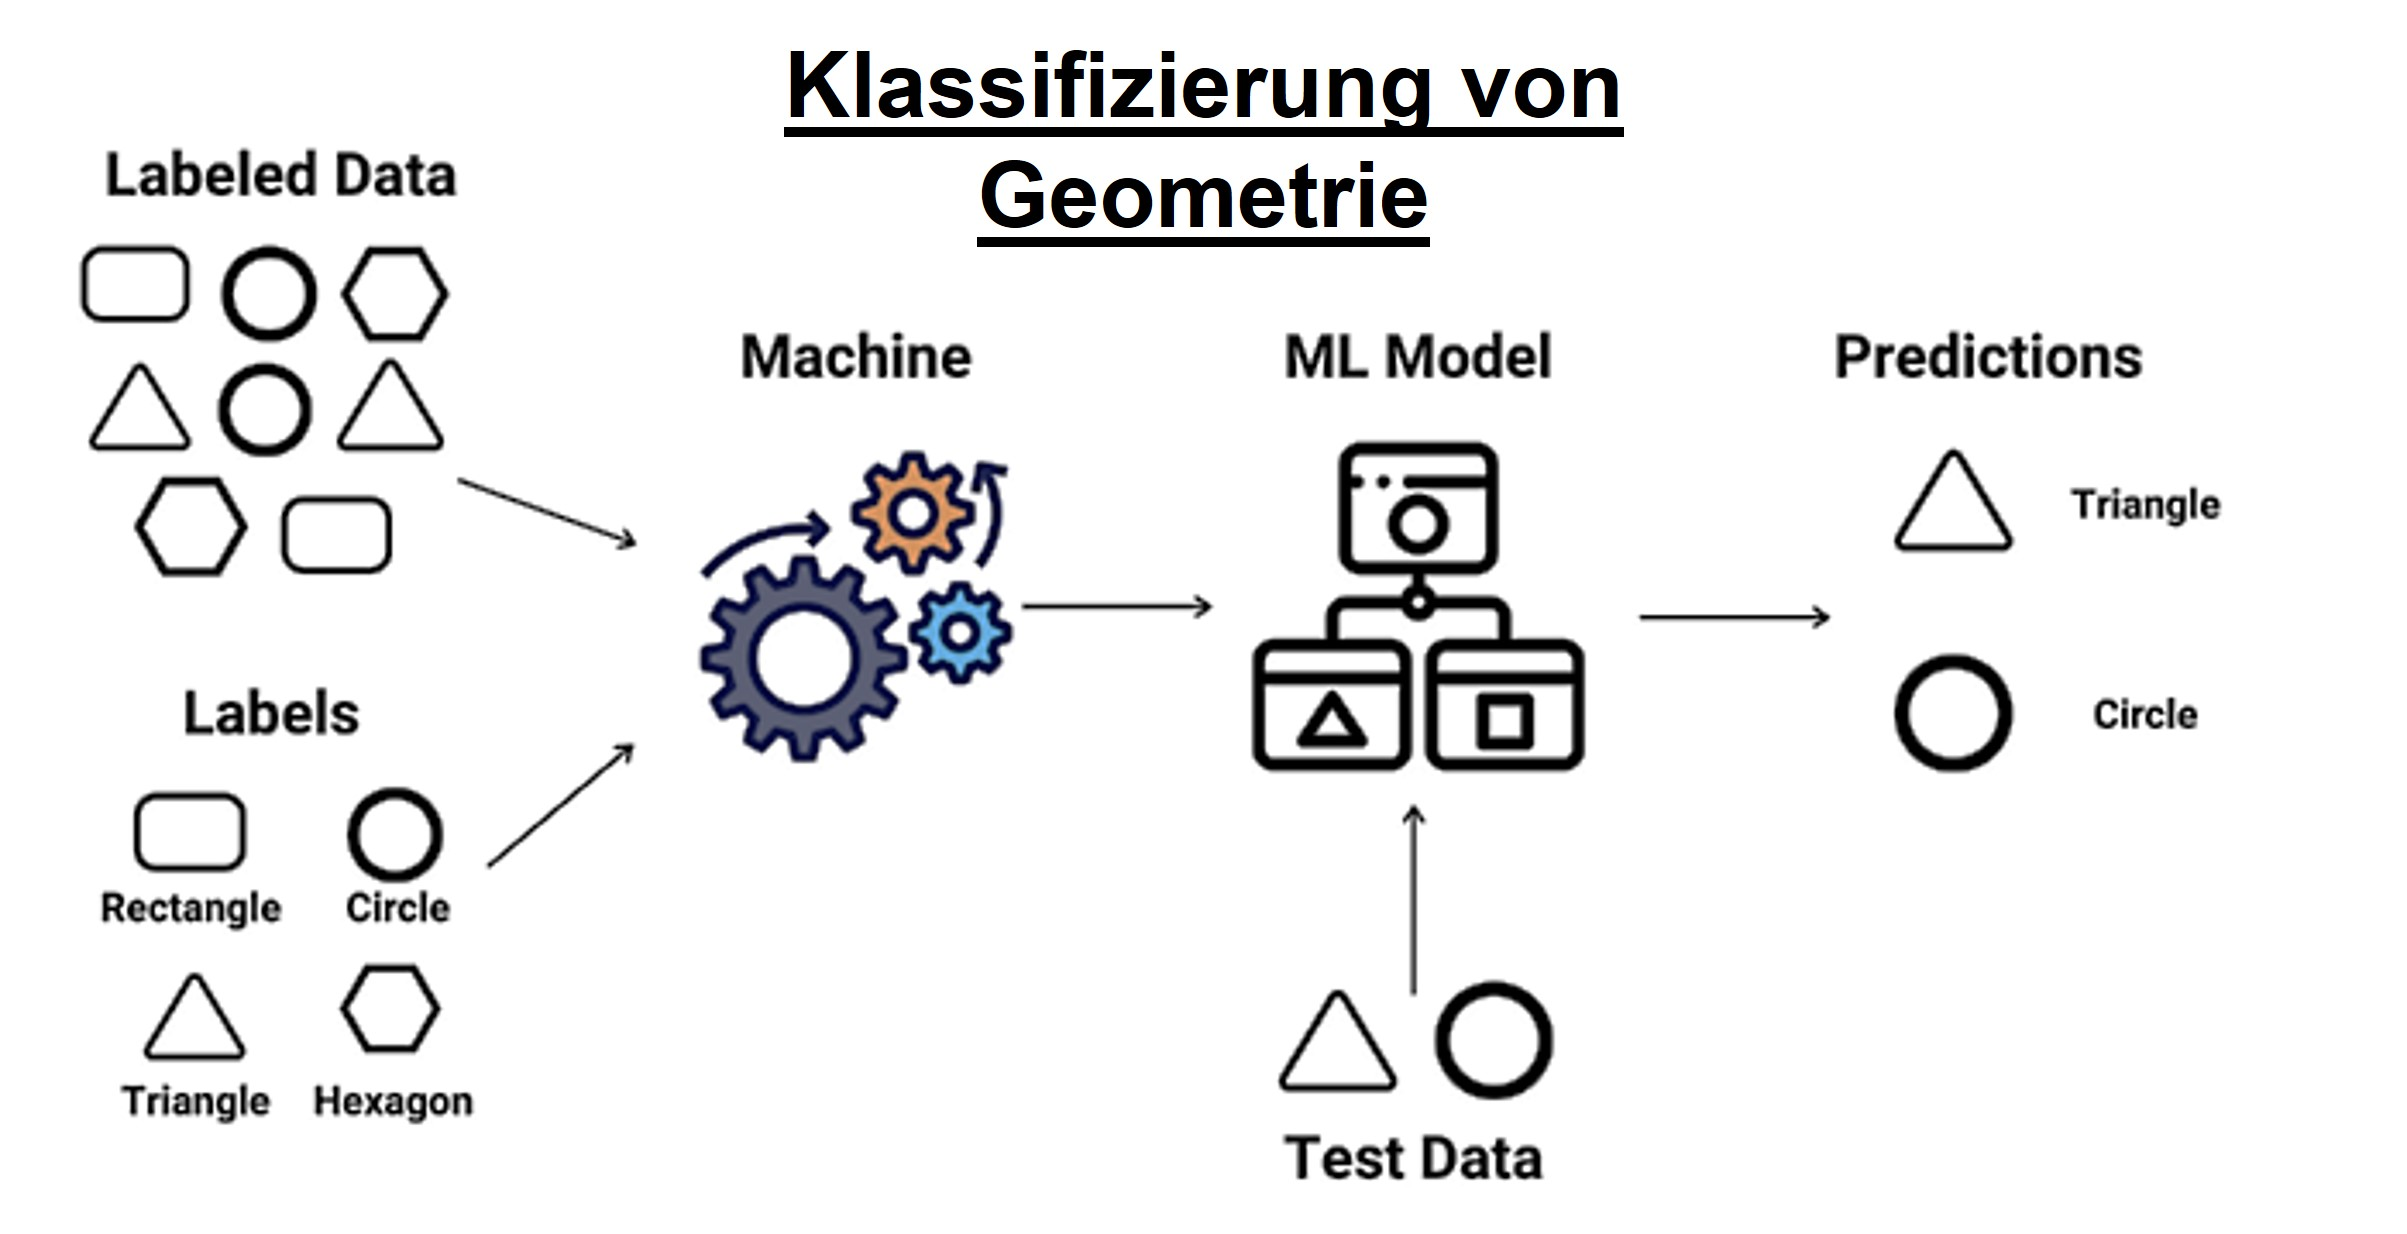
\includegraphics[scale=0.3]{required/supervised_learning.jpg}
			\caption{Beispiel für Überwachtes Lernen [Kozan.2021]}
        	\label{Ground Subtraction}
       	\end{figure}
	\end{frame}

	\begin{frame}{KI-Methoden}{Grundlagen der künstlichen Intelligenz}
		\begin{itemize}
			\item \textbf{Ziel:} Algorithmus zur Bestimmung einer beschreibenden Größe eines Systems, basierend auf im Vorfeld beobachteten Merkmalen dieses Systems, zu finden. Der Algorithmus soll dann auf Fälle angewandt werden, bei denen die Werte der zu beschreibenden Größe unbekannt sind
			\item Wenn pro Beobachtung $N$ Merkmale vorliegen, so werden diese im Vektor $\mathbf{x}$ zusammengefasst
			\begin{equation}
				\mathbf{x} = [x_1,..., x_{N}]^{T} \in \mathbb{R}
			\end{equation}
			\item Die zu beschreibende Größe wird mit $\mathbf{y}$ notiert, die durch den Algorithmus berechnete mit $\hat{\mathbf{y}} = f(\mathbf{x})$.
		\end{itemize}	
	\end{frame}

	\begin{frame}{KI-Methoden}{Grundlagen der künstlichen Intelligenz}
	\small		
	\begin{itemize}
		\item Je komplizierter die Funktion, desto mehr Parameter müssen im Training erlernt werden. Eine simple Beispielfunktion ist die lineare Gleichung. Diese wird im Folgenden noch genauer erklärt.
		\item Gleichzeitig gilt aber auch: Je mehr Parameter erlernt werden können, desto kompliziertere Zusammenhänge können auch dargestellt werden. 
		\item Die Komplexität der Funktion spielt eine entscheidende Rolle für Over- bzw. Underfitting
	\end{itemize}
\end{frame}



	\begin{frame}{KI-Methoden}{Grundlagen der künstlichen Intelligenz}
	\footnotesize		
	\textbf{Over- und Underfitting:}	
	\begin{itemize}
		\item Underfitting bedeutet, dass die Leistung des Algorithmus gering ist. Der Algorithmus ist nicht in der Lage, zu generalisieren.		
		\item Overfitting bedeutet, dass die Leistung des Algorithmus sehr hoch ist, wenn er für die Trainingsdaten ausgewertet wird, aber nicht generalisieren kann.
		\item Gründe für Under- und Overfitting sind unter anderem: die Komplexität des Algorithmus, die Anzahl der Trainingsepochen, mangelnde Diversität der Trainingsdaten.
	\end{itemize}
\textcolor{blue}{**s. curve fitting code**}
	\begin{figure}
		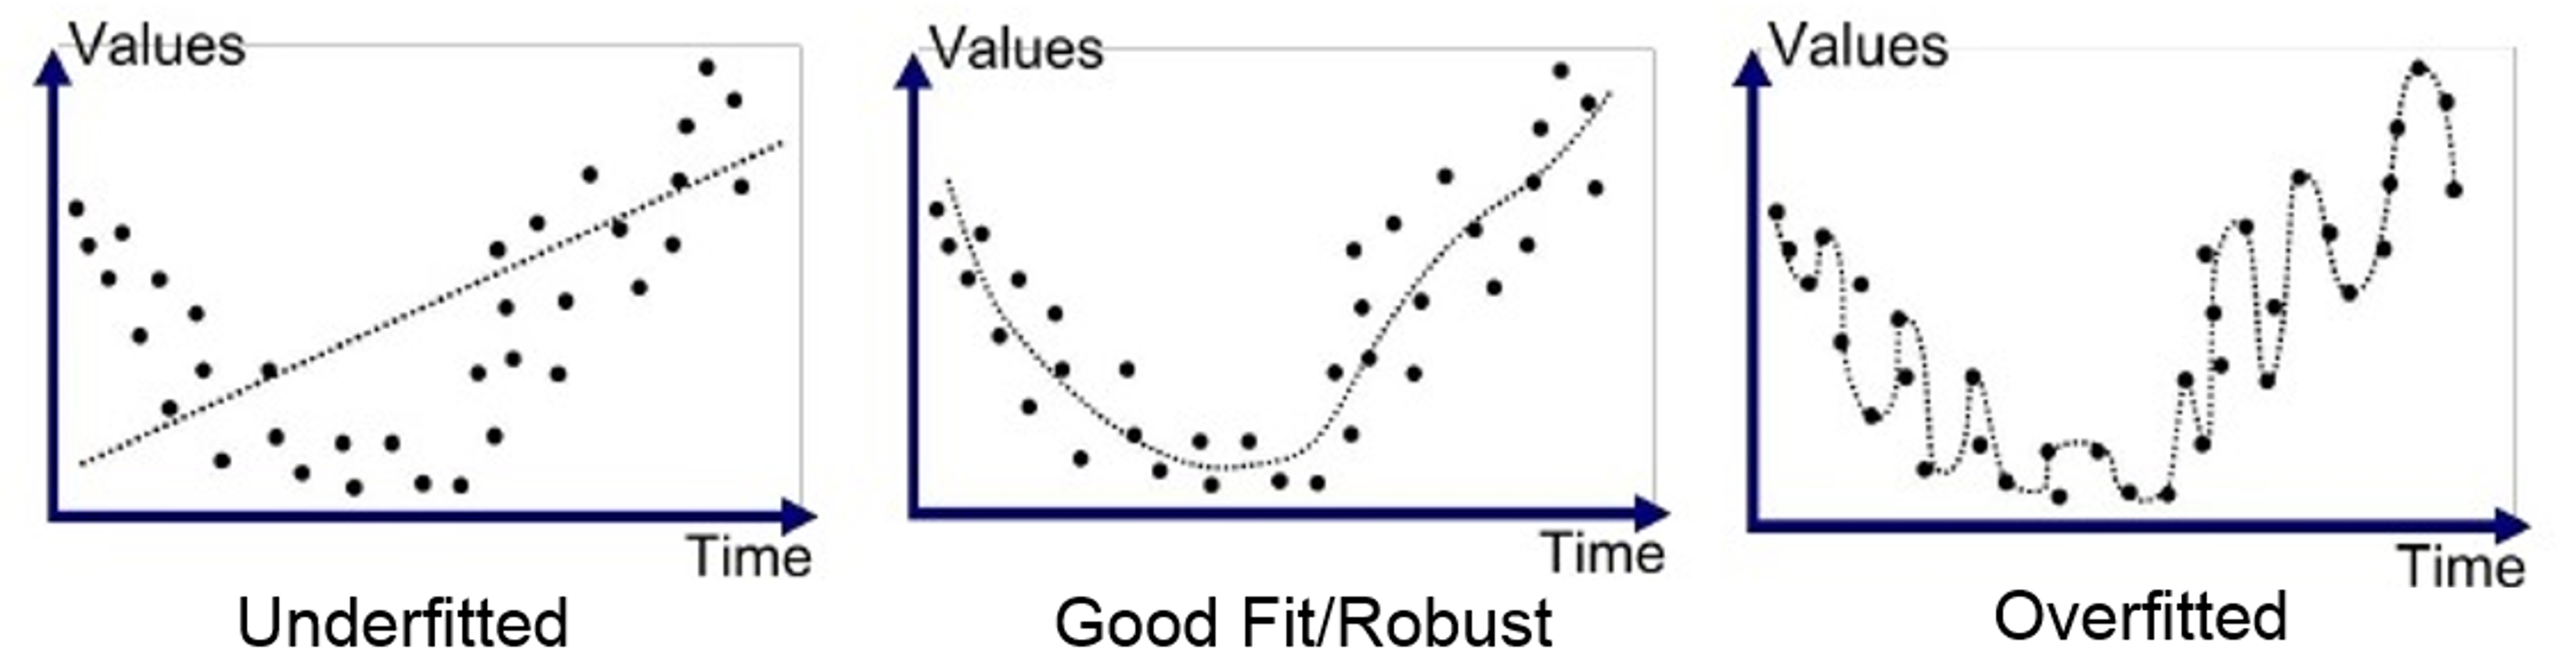
\includegraphics[scale=0.25]{required/Over and Underfitting.png}
		\caption{\scriptsize Beispiel für Overfitting und Underfitting [Bhande.2018]}
		\label{Over and Underfitting}
	\end{figure}
\end{frame}




	\begin{frame}{KI-Methoden}{Grundlagen der künstlichen Intelligenz}
		\textbf{Regression}	
		\begin{itemize}
			\item Falls $\mathbf{y}$ kontinuierliche Werte annimmt, also $\mathbf{y} \in \mathbb{R}$, werden die Eingangswerte $\mathbf{x}$ auf eine Ausgabe $\hat{\mathbf{y}}$ regressiert 
			\item Ziel ist, dass die tatsächliche Lösung $\mathbf{y}$ möglichst gut durch $\hat{\mathbf{y}} $ approximiert wird.
		\end{itemize}			
		\begin{figure}
			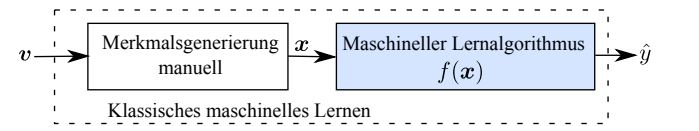
\includegraphics[scale=0.7]{required/Machine Learning.jpg}
			\caption{Regression als Algorithmus des klassischen maschinellen Lernens}
        	\label{Machine Learning}
		\end{figure}
	\end{frame}
	\begin{frame}{KI-Methoden}{Grundlagen der künstlichen Intelligenz}
		\footnotesize
		\textbf{Training: } 		
		\scriptsize	
		\begin{itemize}
			\item Das Lernen basiert auf einer Verlustfunktion und dessen Gradienten. Diese erfasst den Unterschied zwischen dem Ausgang $\hat{\mathbf{y}}$ und dem Zielwert $y$ quantitativ.
			\item Das Ziel des Trainings ist damit, die Funktion $f$ zu finden, bei der dieser Verlust möglichst gering ist. 
			\item Eine häufig verwendete quadratische Verlustfunktion lautet beispielsweise:
			\begin{equation}
				\mathcal{L}(\mathbf{y}, f(\mathbf{x})) = (\mathbf{y} - f(\mathbf{x}))^{2}
			\end{equation}
		\end{itemize}	
		\begin{figure}
			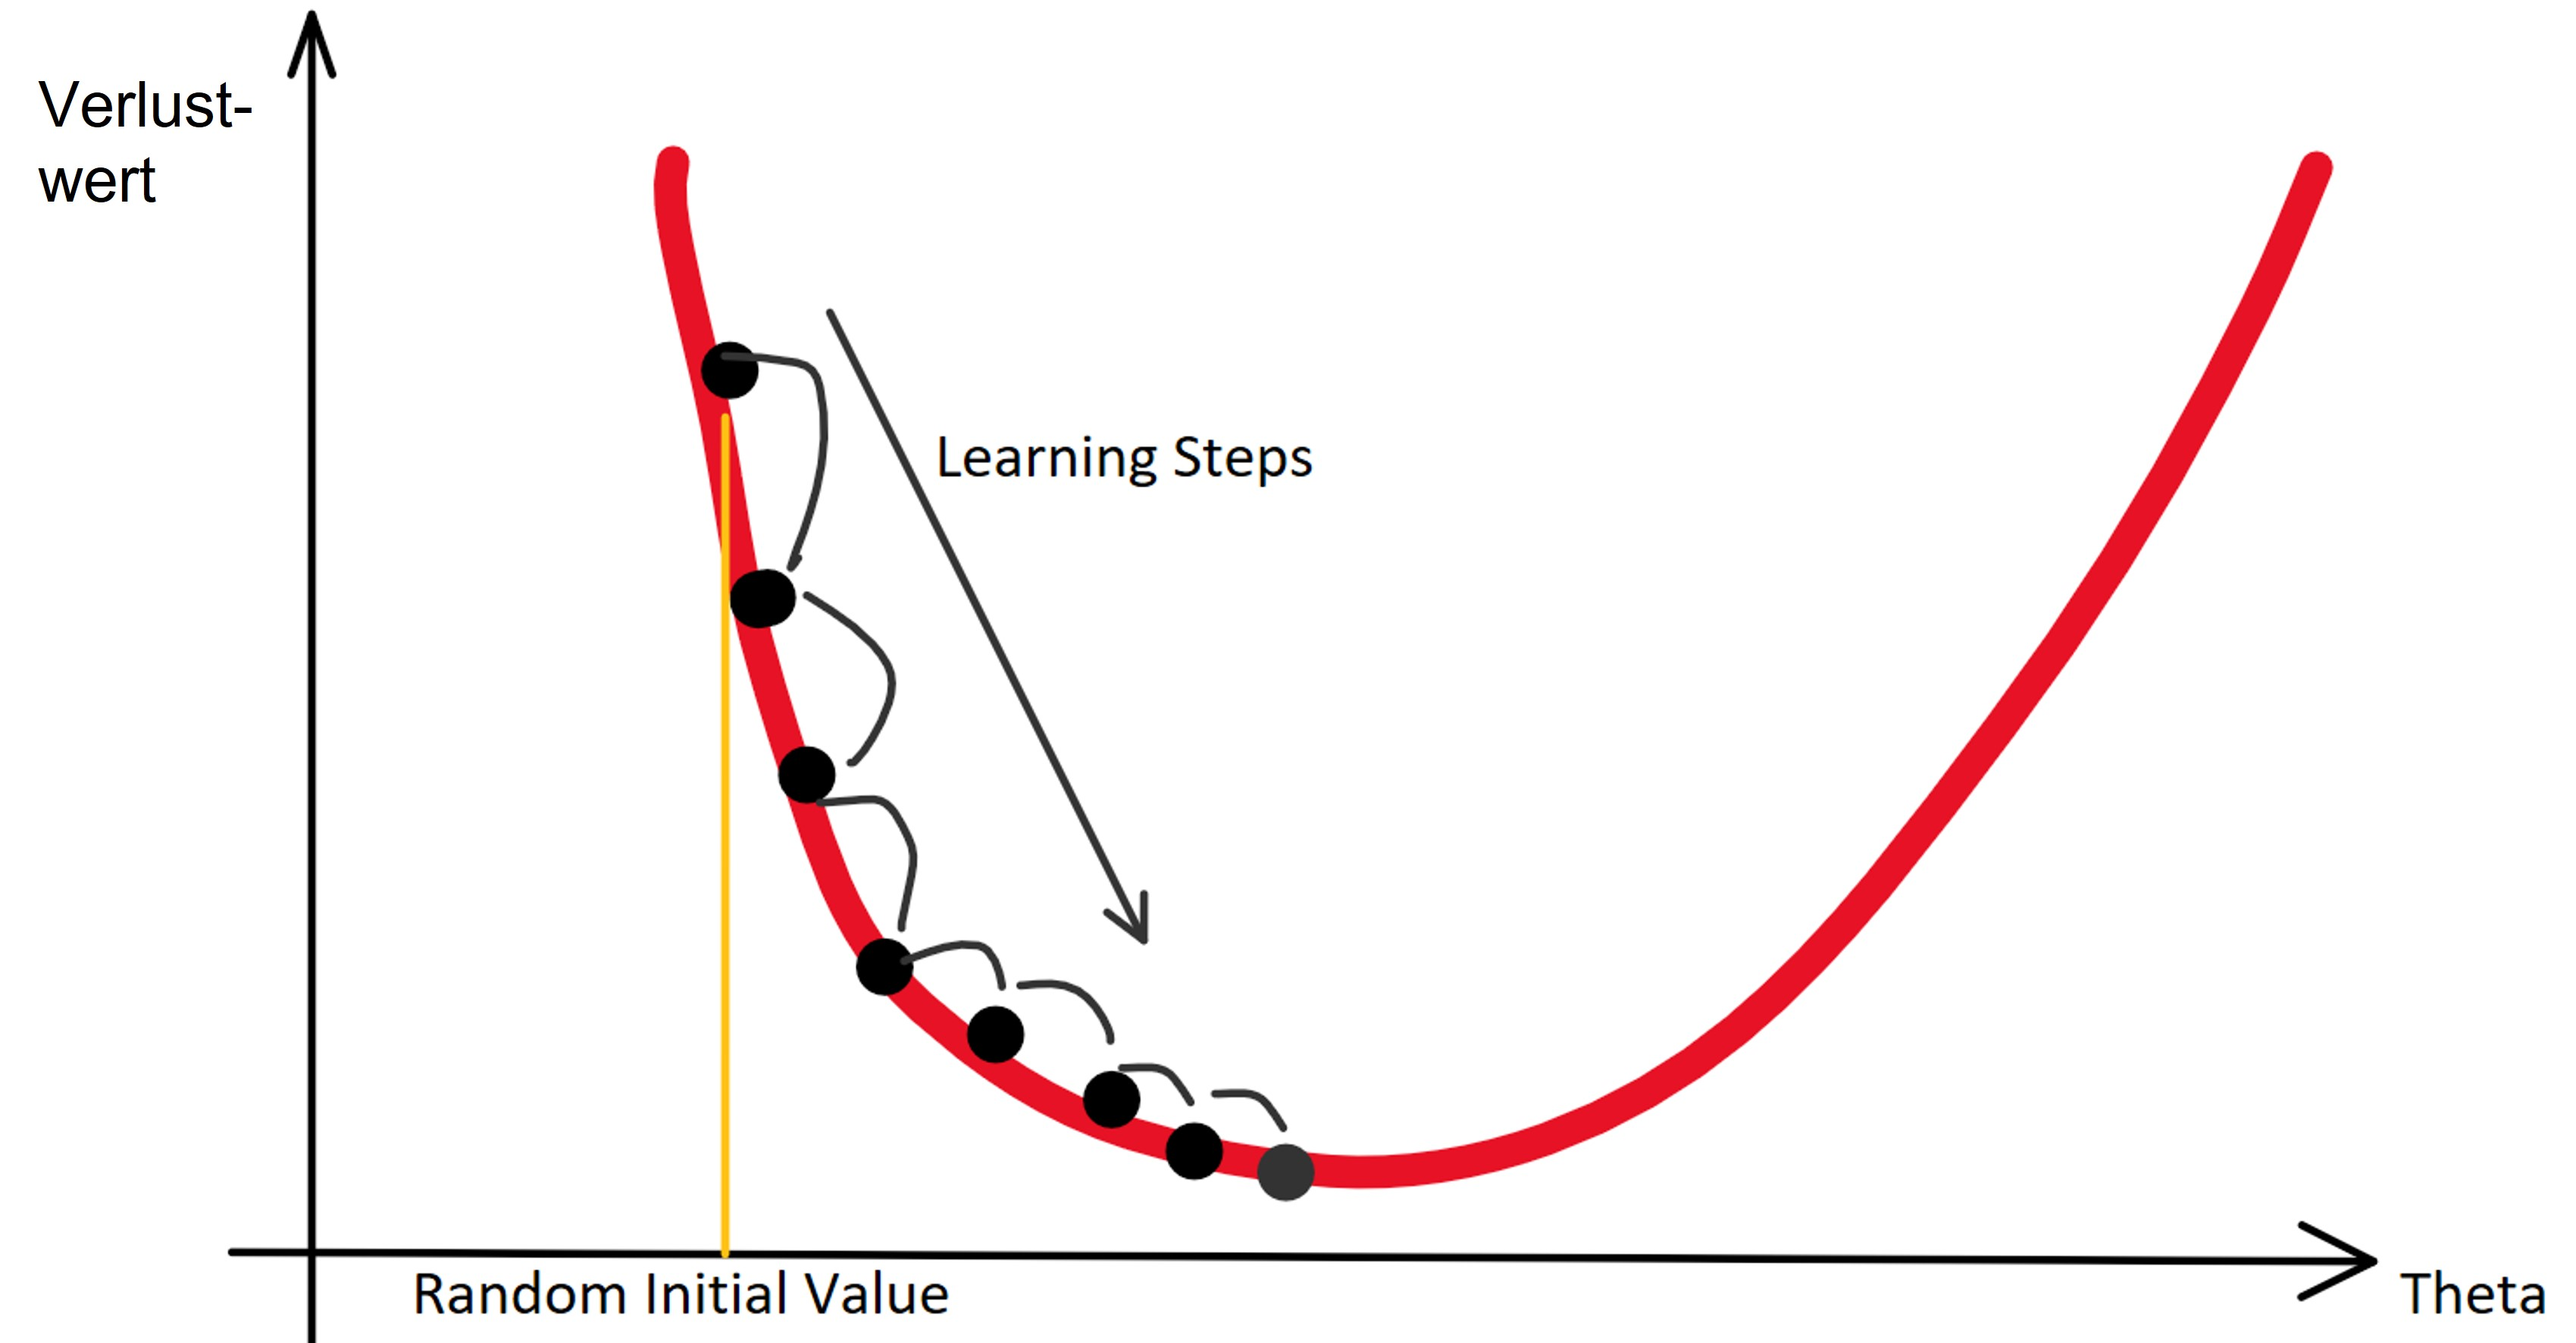
\includegraphics[scale=0.17]{required/Loss_function.jpg}
			\caption{\scriptsize Gradientenabstiegsverfahren [Aunkofer.2019]}
        	\label{Machine Learning}
		\end{figure}			
	\end{frame}

	\begin{frame}{KI-Methoden}{Grundlagen der künstlichen Intelligenz}
	%		\textbf{Umgang mit großen Datenmengen:}
	\begin{itemize}
		\item Falls die Anzahl der Datenpunkte $M$ sehr groß wird, kann es sinnvoll sein den Datensatz im Training in sogenannte Batches aufzuteilen und sich über ein Gradientenabstiegsverfahren sequentiell der Lösung anzunähern.
		\begin{equation}
			\Theta ^{(l+1)} = \theta ^{(l)} - \alpha \frac{\delta}{\delta \theta} \Bigl(\mathcal{L} (y_m, f_{\theta} (x_m))\Bigr) \Big| _{\theta = \theta^{(l)}}
		\end{equation}
		\item[] Dabei ist $l$ der Index der Iteration und $\alpha$ die sogenannte Lernrate, die die Schrittweite pro Iteration festlegt.
		\item Nutzt man für die Aktualisierung der Parameter den gesamten Datensatz $\mathcal{D}$, so nennt man dies eine Epoche.
	\end{itemize}
\textcolor{blue}{**s. gradient descent \& momentum code**}
\end{frame}


	\begin{frame}{KI-Methoden}{Grundlagen der künstlichen Intelligenz}
	\textbf{Normierung}
	\begin{itemize}
		\item Bei der Minimierung des quadratischen Fehlers haben Merkmale $x_n$, deren Wertebereich auch Zahlen mit großem Betrag enthält, einen größeren Einfluss auf die Lösung, als Merkmale, deren Wertebereich nur Zahlen mit kleinem Betrag besteht.
		\item Um dies zu neutralisieren, werden die Wertebereiche aller Merkmale auf das Intervall [0, 1] abgebildet
		\begin{equation}
			x_{n,m}^{\text{norm}} = \frac{x_{n,m} - x_{n,\text{min}}}{x_{n,\text{max}} - x_{n,\text{min}}}
		\end{equation}
	\end{itemize}
\end{frame}


	\begin{frame}{KI-Methoden}{Ermittlung der Kritikalität}
		\textbf{Motivation: }die Kritikalität kann dazu dienen, zu bestimmen, wie kritisch ein bestimmtes Verkehrsszenario ist. Sie kann bei der Entscheidung über die Auslösung von Fahrerassistenzsystemen (z. B. Notbremsung), reversiblem Insassenschutz (z. B. Gurtstraffer) und nicht reversiblem Insassenschutz (z. B. Airbags und Sicherheitsgurt-Pirotecnic) helfen.
		\begin{itemize}
			\item Die Berechnung der Kritikalität ist auch aus Fahrdynamikgleichungen ableitbar und setzt deswegen keine Notwendigkeit für KI-Algorithmen voraus.
			\item Die dadurch gegebene Intuition für das Ergebnis ermöglicht aber ein gutes Verständnis für die Möglichkeiten und Grenzen von KI-Algorithmen.
			\item Ziel ist die kritische Zeit bis zum Auffahrunfall zu berechnen, um z. B. eine Notbremsung zu entwerfen
		\end{itemize}
	\end{frame}






	\begin{frame}{KI-Methoden}{Ermittlung der Kritikalität}
		Ein Maß für die Kritikalität eines Verkehrsszenarios ist die \textbf{\enquote{Time-To-Collision} (TTC)} \\ 
		\begin{itemize}
			\item Je kleiner der Wert der TTC, desto kritischer das Szenario.
			\item Für Auffahrunfälle, die TTC kann aus der Distanz $d$  zwischen beiden Fahrzeugen und der relativen Geschwindigkeit $v_{x,\text{rel}}=v_{x,\text{ego}}-v_{x,\text{tp}}$, die aus der Geschwindigkeit des EGO-Fahrzeugs $v_{x,\text{ego}}$ und der Geschwindigkeit der anderen Verkehrsteilnehmer $v_{x,\text{tp}}$ geschätzt wird, bestimmt werden:
			\begin{equation}
				\text{TTC} = 
				\begin{cases}
					\frac{d}{|v_{\text{x,\text{rel}}}|} \text{ für } v_{x,\text{rel}}<0 \\
					\tau \text{ für } v_{x,\text{rel}} \geq 0 \text{,}
				\end{cases}
			\end{equation}
			\item[] wobei $\tau$ einen großen Wert besitzt, der indiziert, dass das Szenario unkritisch ist.
		\end{itemize}			
	\end{frame}




	\begin{frame}{KI-Methoden}{Ermittlung der Kritikalität}
		\begin{enumerate}
			\item Generieren Sie einen Datensatz $\mathcal{D}_\text{train}$ mit den Eingangsvektoren $x_m$, der die Distanz und relativ Geschwindigkeit zwischen Ego- und vorausfahrendem Fahrzeug enthält. 
			\item Erzeugen sie zudem das zugehörige Label: die TTC. Damit sind die Zufallsvariablen für Ein- und Ausgang:
		\begin{equation}
			x = 			
			\begin{bmatrix}
				d & v_{x,\text{rel}}
			\end{bmatrix}
			^{\text{T}} \in \mathbb{R} 
			\hspace{0.2 cm}
			\text{und}
			\hspace{0.2 cm}			
			y = \text{TTC} \in \mathbb{R}
		\end{equation}
			\item[] Vorgaben bei der Erzeugung des Trainingsdatensatzes $\mathcal{D}_{\text{train}}$:
			\begin{itemize}
				\item Distanz $d$: Schrittweite $1m$; Intervall $[1m, 30m]$ 
				\item Relativgeschwindigkeit $v_{x,\text{rel}}$: Schrittweite $5 km/h$; Intervall $[-60 km/h, -5 km/h]$
				\item $\tau = 60s$
			\end{itemize}			 
		\end{enumerate}
	\end{frame}
	\begin{frame}{KI-Methoden}{Ermittlung der Kritikalität}
		\begin{enumerate}
			\setcounter{enumi}{2}
			\item Erzeugen Sie ein Testdatenset $\mathcal{D}_{\text{test}}$ mit folgenden Vorgaben:
			\begin{itemize}
				\item Distanz $d$: Schrittweite $0.5m$; Intervall $[1m, 40m]$ 
				\item Relativgeschwindigkeit $v_{x,\text{rel}}$: Schrittweite $3 km/h$; Intervall $[-70 km/h, -7 km/h]$
			\end{itemize}
			\item Wenden Sie KI-Methoden an. Bestimmen Sie den Parameter $\theta$ mit Hilfe des Trainingsdatensatzes $\mathcal{D}_\text{train}$. Vergessen Sie dabei die Normierung des Eingangsvektors nicht.
			\item Testen sie den trainierten Algorithmus mit dem Testdatensatz $\mathcal{D}_\text{test}$, indem Sie die Ausgaben $\hat{y}$ mit den korrekten Ergebnissen $y = \text{TTC}$ vergleichen
			\item Visualisieren Sie das das Mapping der KI-Methoden zwischen $d$, $v_{x,\text{rel}}$ und $\hat{y}$. Visualisieren Sie im selben Plot auch den Datensatz $\mathcal{D}_\text{test}$
			\item Integration in die ROS-Pipeline zur Bestimmung der Kritikalität TTC online
		\end{enumerate}
	\end{frame}
			

	\begin{frame}{Quellen}
		Der Aufbau und Inhalt der Folien ist hauptsächlich angelehnt an [Botsch.2020]. Weitere genutzte Quellen sind:
		\begin{itemize}
			\item 1) [Wik.2022] \text{Wikipedia. Lidar. https://de.wikipedia.org/wiki/Lidar. zuletzt abgerufen am 13.05.2022}
			\item 2) [Rummelhard.2017] \text{Lukas Rummelhard, Anshul Paigwar, Amaury Nègre, Christian Laugier. Ground Estimation and Point Cloud Segmentation using SpatioTemporal Conditional Random Field. IEEE Intelligent Vehicles Symposium (IV), Jun 2017, Redondo Beach, United States. pp.1105 - 1110, ff10.1109/IVS.2017.7995861ff. ffhal-01579095}
			\item 3) [GeneSys.2022] \text{ADMA Automotive Dynamic Motion Analyzer with 1000 Hz. 			https://www.leaneautomotive.com/uploads/uMqkUyFj/ProdDescr\_ADMA\_rel\_05.2019.pdf. visited on 13.05.2022} 
			\item 4) [Miller.2022] \text{https://www.wired.com/2014/12/nokia-here-autonomous-car-maps/. Autonomous Cars Will Require a Totally New Kind of Map. visited on 13.05.2022}

		\end{itemize}
\	\end{frame}
	\begin{frame}
		\begin{itemize}
			\item 5) [Breuer.2015] \text{Stefan Breuer, Andrea Rohrbach-Kerl. Fahrzeugdynamik.Mechanik des bewegten Fahrzeugs. 2015. https://doi.org/10.1007/978-3-658-09475-1}
			\item 6) [Hyin.2018] \text{William Hyin. Lidar Obstacle Detection. https://www.codetd.com/en/article/10631576. 2018. zuletzt abgerufen am 13.05.2022}
			\item 7) [Botsch.2020] \text{M. Botsch, W. Utschick. Fahrzeugsicherheit und automatisiertes Fahren. Methoden des Signalverarbeitung und des maschinellen Lernens. 2020. Carl Hanser Verlag GmbH \& Co. KG. eISBN\: 978\-3\-446\-46804\-7}
			\item 8) [Caesar.2020] Caesar et al.. nuScenes: A multimodal dataset for autonomous driving. 2020. arXiv:1903.11027v5	
			\item 9) [Velodyne.2020] Landis Communications Inc.. Velodyne-Lidar-Sensoren ermöglichen 3D-Datenerfassung im neuen NavVis VLX-Kartierungssystem. 2020. zuletzt abgerufen am 13.05.2022
		\end{itemize}
	\end{frame}
\iftrue
	\begin{frame}
		\begin{itemize}
			\item 10) [Bhande.2018] Anup Bhande. What is underfitting and overfitting in machine learning and how to deal with it. https://medium.com/greyatom/what-is-underfitting-and-overfitting-in-machine-learning-and-how-to-deal-with-it-6803a989c76. 2018. zuletzt besucht am 13.05.2022
			\item 11) [Wuttke.2020] Laurenz Wuttke. Machine Learning: Definition, Algorithmen, Methoden und Beispiele. https://datasolut.com/was-ist-machine-learning/. 2020. zuletzt abgerufen am 27.06.2022
			\item 12) [Kozan.2021] Methean Kozan. Supervised and Unsupervised Learning (an Intuitive Approach). https://medium.com/@metehankozan/supervised-and-unsupervised-learning-an-intuitive-approach-cd8f8f64b644. 2021. zuletzt abgerufen am 29.06.2022 
			\item 13 [Aunkofer.2019] Benjamin Aunkofer. Deep Learning. https://data-science-blog.com/blog/2019/01/13/training-eines-neurons-mit-dem-gradientenverfahren/. 2019. zuletzt abgerufen am 29.06.2022 
		\end{itemize}
	\end{frame}
	\begin{frame}
		\begin{itemize}
			\item 14) [ROS.2022] Open Robotics. ROS. https://www.ros.org/. 2022. zuletzt abgerufen am 29.06.2022
			\item 15) [RANSAC.2021] Wikipedia. RANSAC-Algorithmus. https://de.wikipedia.org/wiki/RANSAC-Algorithmus. 2021. zuletzt abgerufen am 29.06.2022
			\item 16) [LinWik.2022] Wikipedia. Lineare Einfachregression. https://de.wikipedia.org/wiki/Lineare\_Einfachregression. 2022. zuletzt abgerufen am 29.06.2022
			\item 17) [NlinWik.2017] Benjamin Aunkofer. Lineare Regression in Python mit Scitkit-Learn. Nicht-lineare Regression mit Scikit-Learn. https://data-science-blog.com/blog/2017/10/17/lineare-regression-in-python-scitkit-learn/. 2017. zuletzt abgerufen am 29.06.2022
		\end{itemize}
	\end{frame}
	\begin{frame}
		\begin{itemize}
			\item 18) [Wang.2019] Bernie Wang. LATTE: Accelerating LiDAR Point Cloud Annotation via Sensor Fusion, One-Click Annotation, and Tracking. 2019. arXiv:1904.09085v1
		\end{itemize}
	\end{frame}

\end{document}

